\chapter{Поляне}

Продолжим про Аланов, но с другой стороны – по русским летописям. Кроме того, попытаемся разобраться, как же на земли полянские пришло название Руси, и какое отношение к сему имеют Варяги.

Общепринятая история невероятно растянута. Вопреки свидетельствам источников, отрицается, что Скифы и Сарматы это прямые предки Славян и даже сами Славяне. Нам навязывают отрывочную картину прошлого. Вспышками фонарика из тьмы кромешной высвечивают то Скифов, то Сарматов, то Славян. Они вдруг возникают на сцене истории, а затем, кроме последних, пропадают без объяснения, не попрощавшись. Наука не сообщает, что происходит в промежутках между этими вспышками, и куда же подевались Сарматы да Скифы, коль они, по науке, ираноязычны и отодвинуты во времени глубже, прочь от Славян.

А по источникам выходит, что Славяне – другое название большой части тех же Скифов и Сарматов. Например даже для Ромеев (жителей той половины Римской империи, которую ученые называют Византией, а славяне именовали Греками), современников княгини Ольги, Скифы это жители Киевской Руси.

Наши летописи странным образом обрезаны по  скифское, сарматское время, а линия отреза разлохмачена множеством вариантов изложения событий. Иноземные источники тоже не шибко радуют нас описанием, происходящего в скифо-сарматском мире до этой линии отреза, да и после. Хроники и летописи затрагивают чужое лишь по мере соприкосновения с ним, а таковым соприкосновением обычно является война или торговля.

Итак, внутренние источники сгинули, внешние скудны. Будто вырван кусок истории, кусок, захвативший определенную местность на протяжении некоторого времени.

Однако существует еще Бермудский треугольник, составленный из Славян, Русов и Варягов. Какое отношение имеют Славяне к Русам, а Русы к Варягам? Вот уже несколько сотен лет ученые спорят, разделившись на два непримиримых лагеря – норманистов и антинорманистов. Последним даже в толковом названии отказали, произведя его от первых.

Норманисты утверждают, упрощенно говоря, что государство Киевская Русь основано норманами – скандинавами. Это призванные княжить над Славянами Варяги – Рюрик с братьями, да его потомство и родичи. Антинорманисты же полагают, что Рюрик был из Славян с южного побережья Балтийского моря.

У представителей обеих научных школ на руках одинаковый набор источников, главнейшие из которых, да и, что кривить душой – единственные письменные – это русские летописи. Нигде кроме них про Рюрика не сказано\footnote{В середине и второй половине 9 века, однако, по страницам хроник вроде Annales Bertiniani и Annales Xantenses гуляет северянин Рорик, племянник короля большей части Дании – Ютландии, Харалда «Клака» Халфданссона. Рисковый, стремящийся к власти человек, Рорик обрел её, захватив Дорестад (Dorestad, около нынешнего голландского города Wijk bij Duurstede). В 873 году Рорик появляется в хрониках в последний раз, чтобы присягнуть на верность Германскому королю Хлудовику. Этого Рорика некоторые исследовали отождествляют с Рюриком.}, значит, надо прочесть и рассудить. Однако нас подстерегает опасность.

Общепринятые представления, укоренившиеся в разуме, искажают смысл слов, вложенный летописцем. Какими вам видятся Варяги? Эдакими патлатыми викингами с топорами, да еще в рогатых шлемах? Что в этой картине обосновано? Проверим.

Почему Варяги – непременно викинги? Потому, что так говорят ученые-норманисты. Вероятно, они записывают всех скандинавов в викинги. Но викинги это морские разбойники у скандинавов. Разве все скандинавы были разбойниками?

Почему шлемы рогатые? Так художники рисуют и в фильмах показывают. Но у викингов не было рогатых шлемов. Задача шлема – отводить удар в сторону, а не задерживать его рогами. Рогатых шлемов в Скандинавии найдено всего пара штук, и те надевались для справления обрядов.

А что насчет длины волос? Сходный вопрос про давних Славян – каковы из себя? Ну мирные жители ладно, с какой угодно прической, хотя обычно «под горшок». Однако воины всегда, во все времена, даже сейчас, стригутся коротко или налысо. Поэтому когда на картинке или в кино показывают длинноволосых воинов, это неправдоподобно. Верно показан полководец, князь Святослав – налысо бритый с оселедцем. Казаки такие же. В Радзивилловской летописи есть картинка – с русского витязя слетает шлем, а под шлемом лысая голова. 

От Рима до Руси воины стриглись коротко либо брились. Ибо волосы в бою мешают. Вон амазонки одной груди лишались, чтобы лук удобнее вешался и снимался, а тут какие-то воинственные мужики отращивают себе роскошные кудри ниже плеч. На средневековых изображениях, викинги имеют короткие волосы, кое-кто носит короткие бороды, многие лишены бород и усов. Что им, бородой рыбу с борта ловить?

У некоторых народов длинные волосы вообще имела только знать. Когда Бургунды убили короля Франков, Хлодомира, то узнали его по волосам до плеч, ибо правители Франков не стриглись и причесывались на прямой пробор\footnote{Франки – не самоназвание. По преданию, это были потомки разгромленных, отступивших Троянцев. Другие имена давних Франков: Приам, Антенор, Сунно, Маркомир, Фарамунд, Хлодио, Меровей, Хлотар.}. Тамошние простолюдины же стриглись в кружок, а носить долгие волосы им запрещалось.

Или вот ученые пишут в своих работах – «славянские племена». Либо – «балтийские племена». Что под словом «племя» разумеют ученые? Они не задают себе такой вопрос. Просто используют слово, вкладывая в него нечеткий смысл. Попроси пояснить, в ответ получишь туманные высказывания. Но ведь язык науки должен быть точным! А выходит, что ученые зачастую не вкладывают в произносимое четкий смысл.

Словом «племя» широко пользуются и в переводах древних исторических сочинений. Например, в подлиннике стоит латинское «nation», то бишь «народ», а переводчик нам толкует – «племя». Или, латинское «gens», тоже «народ», у переводчиков опять-таки «племя». Хотя в случае «gens» можно с нятяжкой переложить как «племя» в уточняющем выражении вроде «gens fortissima Sclavorum» – «могучее Склавское племя», когда речь идет о принадлежности некоего могучего народа к Скла\-вскому роду («gens»). Ни современные ученые, ни переводчики – а древние исторические сочинения переводят обычно те же ученые – этих тонкостей не знают и не чувствуют.

Хорошо. Что первым делом воображаешь, когда слышишь слово «племя»?

Наверное, единицу общественного строя вроде как у киношных туземцев тропического леса. Лезешь себе через джунгли, рубишь лианы острым мачете. Поперек лежат бревна, с ветки свисает питон, показывая бледно-розовый раздвоенный язык. Тут бац – выходят диковинно изукрашенные, с копьями настороже, люди. Они не понимают вашу речь! Жестами поясняют, что вы вторглись на их землю. Надо потолковать. Вас ведут тайными тропами. Чаща раздвигается. Увенчанный черепами частокол, за ним хижины. Тут живет племя. В самом большом шалаше сидит вождь в нелепой, с европейской головы, фетровой шляпе. Хук!

Такое ли было общественное устройство у Славян до пришествия варяжских князей? Упоминания о проведениях вече в позднейшее время, да и положение самих князей на первых порах, указывают на иное. Князья, если только не брали власть силой, поначалу были наемными или выборными руководителями, и соблюдали законы общества, в котором жили. Летописи пестрят намеками на принятие Славянами решений сообща –  Древляне совещаются, Киевляне созывают вече. 

Так какие были славянские племена? А может ученые что-то путают? Где написано про славянские племена? В летописях не написано.

Как же... Ученые основывают свои соображения на летописях. Не потрудившись принять во внимание четкий смысл, вкладываемый летописцами в слова «племя», «народ», «язык». Слова эти в летописях имеют совсем иные значения, нежели в современных научных, а зачастую и богословских работах.

Только поняв исконное значение слов, мы уразумеем, что написано в летописях. Задача, покамест, не выяснить некую истину – как было на самом деле – но что именно сказал летописец, что имел в виду.

Языком раньше именовали не набор слов, присущий определенному сообществу людей, но ветвь родового сообщества. Как языки пламени исходят из общей основы, так и языки племени. Такой, отделившись от корня, образует народ, в своем краю – чужом либо части исконного. Народ – те, кто народились в такой-то земле, населяют ее. Народ может получить название, отличное от исходного. Упрощенно говоря, Англичане переселились в Америку и стали Американцами.

Давний смысл слова «язык» ускользает от ученых (историков, языковедов) и некоторых сочинителей христианских произведений, которые упорно трактуют «язык» как набор слов, хотя даже в Библии «язык» употребляется именно в значении ветви рода.

Но двинемся дальше. «Племя» означает, буквально, родственников, у которых общие предки. Отсюда – племянник, племянница. Племя – те, кто расплодились. Единица племени – плод.

«Колено» значит – отколотое, часть. Колено племени – часть племени. А вот «поколение» – это родичи, следующие за «околевшими», умершими. Поэтому поколение, по околению.

Согласно преданию, попавшему в состав Библии и перешедшему в летописи и саги, у Ноя было три сына – Сим, Хам и Афет. От них пошли потомки, племена – Симово, Хамово, Афетово\footnote{Примечательно, как в некоторых русских летописях вместо строки «яко благословил праотец наш Ной прадеда нашего Афета» сказано «прабабыш» вместо «праотец» и «прабаба наша» вместо «прадеда нашего».}. Когда летописец говорит, что такой-то народ – племени Афетова, значит, сей народ относится к племени указанного родоначальника, произошел от такого-то начального предка.

После всемирного потопа Сим, Хам и Афет разделили между собой земли. В Повести временных лет перечень, кому какие земли достались и кто их населяет, существенно шире, чем в известном нам тексте Библии, и более подробен, нежели в Хронике Георгия Амартола (9 век), которую считают одним из источников Нестора. То бишь Нестор привлекал другие, более полные источники. Амартол, вероятно, просто использовал их же. Таковые, в разных вариантах, встречаются в греческих церковных сочинениях.

Повесть временных лет начинается преданием про разделение стран между сыновьями Ноя. Почитаем Ипатьевский список. Я буду делать оттуда выдержки, по ходу останавливаясь и трактуя, как понимаю. Названия переводить на современные не стану. Здесь и далее, под летописными Словенами понимаются Славяне.

Сперва говорится, какие страны кому «принадлежат», причем по именованиям можно догадаться, что это частично переписывалось из греческого источника невесть как давнего по отношению к летописцу. Названия некоторых стран одноимённы с народами, однако неясно, проживают ли в них эти народы во время летописца. По старой памяти страна, населенная другими, могла сохранять прежнее имя.

\begin{quotation}
Яся всток Симови: Перьсида, Ватр, доже и до Иньдикия в долготу и в ширину и до Нирокурия, якоже рещи от встока доже и до полуденья\footnote{До юга.}, и Сурия, и Мидия и Ефрат реку, и Вавилон, Кордуна, Асурияне, Месопотамия, Аравия старейшая, Елумаис, Индия, Аравия силная, Кулии, Комагины, Финикия вся.

Хамови же яся полуденья страна: Егупет, Ефиопья, прилежащия к Индом, другая же Ефиопья, из нея же исходит река Ефиопьская Чермьна, текущия на въсток, Фива, Луви прилежащи доже до Куриния, Мармариа, Сурите, Ливуи другая, Нумидия, Масурия, Мавритания противу сущи Гадиру. Сущим же к встоком имать Киликию, Памфилию, Писидию, Мосию, Лукаонию, Фругию, Камалию, Ликию, Карию, Лудью, Масию другую, Троаду, Солиду, Вифунию, старую Фругию; и островы пакы имать: Сардинию, Крит, Купр, и реку Гиону, звоему Нил.

Афету же яся полунощныя\footnote{Северные.} страна и западная: Мидия, Ольвания, Армения малая и великая, Каподокия, Фефлагони, Галатия, Кольхыс, Воспории, Меоти, Дереви, Сармати, Тавриани, Скуфия, Фраци, Македония, Далматия, Молоси, Фесалия, Локрия, Пеления яже и Полопонис наречеся, Аркадия, Ипириноя, Илурик, Словене, Лухития, Аньдриакия, Аньдриатиньска пучина; имать же и островы: Вританию, Сикилию, Евию, Родона, Хиона, Лезвона, Куфирана, Закуньфа, Кефалинья, Ифакину, Керкуру, часть Асийския страны, нарицаемую Онию, реку Тигру, текущую межю Миды и Вавилоном;

до Понетского моря на полнощные страны, Дунай, Днестр, и Кавькасинския горы, рекше Угорьскыя\footnote{Как видим, Кавказ, а не Карпаты, соотнесены здесь с Угорскими горами.}, и оттуда рекше доже и до Днепра; и прочая реки: Десна, Припеть, Двина, Волхов, Волга, яже идет на всток в часть Симову.
\end{quotation}

Нестор различает Сарматов, Скифов, Словен, Тавриан, Меотов. По греческим источникам, в этой части предания, Словене и Дереви (Древляне?) не встречаются, хотя есть Скифы и Сарматы. Вижу два варианта, почему так. Первый – в греческих хрониках из предания убраны «Склавины». Второй – они же известны грекам как Скифы и Сарматы.

Самоназвание царских Скифов было, по Геродоту, «Сколоты». Похоже на «Кельты»? Предположение замечательно, ибо сердцем Гальштатской (Холлштаттской) культуры, соотносимой с исходными, ранними Кельтами, есть область, где жили Норицы или Норцы, которых Нестор отождествил со Словенами. В корне самого названии города Холлштатт, по которому названа культура, чувствуется слово «Сколоты». Выпадение букв «л», «с», и смена «к» на «г», разница между коими меньше игольного ушка, всюду вскрывает тождество либо родство.

Шотландцы, они же Ск\'оты (Скотты) – Готы. Готы, они же Геты – Кельты. Скифы, Скиты – Скоты. Скоты – Сколоты. Усматривая сходство между «Склово» и «Сколо», в Склавенах (Скловенах) и Сколотах, я не решаюсь сделать вывод.

Поскольку источник у Нестора греческий и старый по отношению к нему, печерский монах мог дописать Словен и Дерев по соображению, что они тоже живут в северной части. Или дописал по другой причине. Таким образом количество стран увеличилось, а Словене отмежевались от Скифов и Сарматов. Далее летописец приступает к описанию языков (ветвей племени), населяющих земли Афета, и приводит данные, которых Греки не сообщают. Прочтите следующее, держа в памяти, что с Варяжским морем обычно сопоставляют Балтийское, но всегда ли такое отождествление верно?
 
\begin{quotation}
В Афетови же части седять: Русь, Чудь и вси языце\footnote{По ряду списков: «и си языци».}, Меря, Мурома, Весь, Мордва, Заволочьская Чудь, Пермь, Печера, Ямь, Угра, Литва, Зимегола, Корс, Сетогола (Летьгола), Любь. Ляхове же и Пруси и Чудь приседять к морю Варяскому;

по сему же морю седять Варязи семо к востоку до предела Симова, по тому же морю седять к западу до земли Агаляньски и до Волошьскые.

Афетово бо и то колено: Варязи, Свеи, Урмане, Готе, Русь\footnote{Гти-русь в Воскресенском списке.}, Агляне, Галичане, Волохове, Римляне, Немце, Корлязи, Венедици, Фрягове и прочии приседять от запада к полуденью и сседяться с племянем Хамовым.
\end{quotation}

Отдельными языками (ветвями племени Афета) названы, кроме прочих, Русь, Пруси, Свеи и Варяги. Про Свеев – разговор особый, отложим до поры до времени. 

Варягам летопись отводит место по морю Варяжскому, причем к востоку до «предела Симова» – до земель Сима, и на запад к «земле Аглянской и до Волошскые».

Насколько это применимо к Балтийскому морю, коль оно, как считают, постоянно равно в источниках Варяжскому?

Предел Симов это же восток. Вспомним:

\begin{quotation}
Яся всток Симови: Перьсида, Ватр, доже и до Иньдикия в долготу и в ширину и до Нирокурия, якоже рещи от встока доже и до полуденья, и Сурия, и Мидия и Ефрат реку, и Вавилон, Кордуна, Асурияне, Месопотамия, Аравия старейшая, Елумаис, Индия, Аравия силная, Кулии, Комагины, Финикия вся.
\end{quotation}

А западная граница, до которой сидят Варяги? Земли Аглянские и Волошские. Волохами, Влахами называли некий народ, что обитал в разные времена в нынешней Болгарии, Боснии, Молдавии, Трансильвании, короче говоря на Балканах и около.

Какое море граничит с Балканами на западе, и пределом Симовым на востоке? Не Балтийское, но Черное.

Таким образом, в летописи, под Варяжским морем сначала подразумевается Балтийское, а затем – Черное. Это совершенно путает рассуждения, ибо порой неясно, какое море надо понимать под Варяжским.

Однако вопрос, где именно живут Варяги, о которых говорится:

\begin{quotation}
по сему же морю седять Варязи семо к востоку до предела Симова, по тому же морю седять к западу до земли Агаляньски и до Волошьскые.
\end{quotation}

Речь может идти как о северном побережьи Черного моря, так и об южном, ныне зовущемся Турцией, а ранее Малой Азией, составленной из множества держав.

В другом списке, при перечислении народов сказано:

\begin{quotation}
Мы же глаголем по речи языка своего, иже от Афета языцы изыдоша в части его живут: язык варяжский, словенский, чудь, ямь, лопь, пермь, корела, печера, югра, литва, явтези, пруси, нерьдва, меря, мордва, мещера, мурома, корс, зимигола, ливь. 
\end{quotation}

«Речь» – вот слово, которое мы теперь заменили «языком». Речь языка своего, наречие – набор слов, присущий языку (ветви племени). К племени Афета отнесены языки, ветви: Варяги, Словены, Чудь, Ямь и так далее.

Но перечень афетовых языков может быть и таким:

\begin{quotation}
От афета же и суть рождшеся языки, иже в столпотворение разделенни язык быша: мидои; кападокеи; галатии, же суть икатеи; еллины, иже есть анос; фетатилои; клакои; фракеи; македонни; сартамате; роднои; армении; сиколои; норица, иже суть словене; руними, иже зовутся грецы. Сии же суть афетови языцы, третияго сына Ноева.
\end{quotation}

Греческий вариант по «Летописцу Эллинскому и Римскому» свода 15-го века выглядит так: 

\begin{quotation}
Племя Афетово. Регма, от него же иудеи. Ефиопьскаа страна. Гамер, от негоже скуфи, Мадии, от негоже миди, Иоанус, от негоже Ионес, Иелиса, от негоже Оли, Фовел, от негоже авери, Момосу, от негоже каппадоци, Фарис, от негоже фраци, Асханос, от негоже Ригинес. Риффа, от негоже пефлагони, Фургам, от негоже фруге, Фаусис, от негоже Киликис, Фитин, от негоже купряне, Китию, Роди, Угог, от негоже готфе, Сесмада, от негоже римляне.

Афетова часть. Афету же 3-му сынов: Колху, Меланехлену, Сапрамате, Герману, Сарамате, Неоте, Иехуте, Таире, Фраке, Вавустрану, Илурии, Македонес, Елинес, Ливиес, Фругиес, Панонеу, Несториу, Уену, Давние, Иапкес, Калавру, Пику, Латину, иже суть римляне, Тури, Гане, Галате, Ливусте, Камьпану, Велтиверьс, Галу, Акунтину, Луиану, Вантес, Катану, Лиситану, Аукеку, Вретанику, Скоту, Спану.
\end{quotation}

Так многие народы, известные нам по греческим дохристианским источникам, уже в христианских хрониках получили привязку к библейской родословной. Но древние Греки о Ное и его сыновьях молчат. У Греков от Потопа спасся другой человек – сын Прометея, Девкалион. Однако по ветхозаветным представлениям, уцелела только семья Ноя, поэтому надо было все народы произвести от него. Принимая во внимание хорошо проработанную в Библии родословную, думаю, что Ной и его потомство некогда действительно существовало. Другое дело – его связь с упомянутыми народами. Чего кстати в каноне Библии нет.

Хорошо отношение колена, языка и племени видно по такому отрывку из русских летописей:

\begin{quotation}
От Афетова же колена сына Ноева бысть 20 язык, в них же бе и наш Словенский от Афетова племени.
\end{quotation}

То бишь колено Афета имеет 20 отростков – языков, среди коих и Словенский язык (не набор слов, но отросток, отдельная часть племени Афета). Я настойчиво твержу это и повторяюсь, чтобы сейчас, в этой главе, переменить современное восприятие слов на летописное. Итак, язык – не набор слов, но ветвь, часть племени.

Перечни языков в разных списках – различны. Сие наводит на соображения. Может, одни перечни краткие, а другие расширенные. Либо, некоторые названия даны в переводе или другом варианте. Возможно и такое – для части языков приведены одновременно несколько именований, скажем, по два на один язык.

Библейское предание, изначально, вероятно, освещающее отрезок истории одного рода кочевников, стало трактоваться как отрезок истории всего рода человеческого и дополнялось уже по этим соображениям. Мне важно выяснить, какие «языки» – народы – знал Нестор, и я оставляю в стороне привязку народов к потомкам Ноя.

Продолжим чтение Повести временных лет по Ипатьевскому списку. Летописец возвращается ко времени, когда человечество еще не было разделено на «языки»:

\begin{quotation}
Сим же, и Хам, и Афет, разделивше землю, жребье метавше не преступати никомуже в жребий братень, живяху кождо в своей части. Бысть язык един, и умножившемся человеком на земли, помыслиша создати столп до небесе, в дни Нектана и Фалека; и собрашася на месте Сенар поли здати столп до небесе и град около его Вавилон, и создаша столп за 40 лет, несвершен бысть.

И сниде Господь Бог видети град и столп, и рече Господь: се род един и язык един. И смеси Бог языки, и раздели на 70 и 2 языка, и разсея по всей земли.
\end{quotation}

Итак, до строительства Вавилонской башни, столпотворения, земли уже разделены между братьями, и народы этих братьев обитают по своим землям – так в Библии и у Нестора. В предании заложено противоречие, ибо сначала говорится, что народы от разных братьев уже заселили местности, а потом оказывается, что после столпотворения они «рассеиваются» по всей земле. 

Возможно, слово, переведенное как «рассеивать», означало нечто иное. В Библии понятия «язык» и «наречие» разделены, однако при «смешении» (еще одно непонятное мне употребление слова) языков люди разных народов, строящих башню в Вавилоне, вдруг перестали понимать наречия друг друга и поэтому прекратили строить башню. Предполагается, что эта башня – зиккурат Этеменанки с храмом богу Мардуку, покровителю города.
   
Происходит разделение единого народа, языка, на 72 отдельных. Возможная трактовка – деление на 72 административные единицы. Восточные части принял Сим. Южные – Хам. Северные и западные – Афет:

\begin{quotation}
По разрушению столпа и по разделении язык, прияша сынове Симови восточные страны, а Хамови сынове полуденьные страны, Афетови же прияша запад и полунощныя страны. От сих же 70 и дву языку бысть язык Словенск от племени Афетова, нарицаемеи Норци, иже суть Словене\footnote{Татищев дополняет: «жили близ Сирии и Пафлагонии».}.
\end{quotation}

К этим 72 частям принадлежала и Словенская часть, Словенский язык, они же Норцы.

В давних источниках, включая карты, возле Италии через Альпы, лежит страна Норикум или Норицы. Народ ее зовется тоже Норицы или Нори. Города Норикума и координаты оных помещены в «Географии» Птолемея. Плиний в «Естественной истории» сообщает, что Норики живут в Карнийских Альпах (ныне на границе Австрии и Италии) и раньше назывались Таврисками. Соседний с Нориками народ, по Страбону – Венделики. Они же, по моему разумению, в разных местностях, временах и говорах – Венеды, Венды, Венеты, Ванды, Энеты, Анты. Иордан в «Гетике», впрочем, разделяет Венетов, Антов и Склавенов, отмечая, что происходят они от общего корня – Венетов.

И вот Нестор пишет – ветвь Афетова племени, Норцы или Словены, стала расселяться. Из своей исходной земли Словены обжили реку Дунай, а от Дуная произошло дальнейшее распространение Словен по другим землям, при этом получая отдельные названия:

\begin{quotation}
По мнозех же временех сели суть Словени по Дунаеви, где есть ныне Угорьска земля и Болгарьска. От тех Словен разидошася по земле и прозвашася имены своими где седше на котором месте: яко придешде седоша на реце именем Морава и прозвашася Морава, а друзии Чеси нарекошася; а се ти же Словени Хровате Белии, и Сереб, и Хорутане. 
\end{quotation}

Таковые «отдельные» Словены, как Чехи, Морава, Сербы и так далее следует считать, во-первых, «народами». Не племенами. Племён всего три – Афета, Хама и Сима.

Однако, названия народов – Чехов, Сербов, прочих в летописи имеют и другое значение. Стр\'аны. Чехи – имя не только народа, но и населяемой им страны. Чем отделяется одна страна от другой? Границами. Следовательно, существовали границы.

И вот в страну Дунайских Словен пришли Волхи. Слово «насплящем», я перевести не могу. Ученые считают, что это «прогнали», однако я не делаю выводы так легко. После пришествия Волохов часть Словен перебралась на Вислу, и стала зваться Ляхами:

%, а Ляхи прозвали соседние народы Полянами, Лутичами, Мазовшанами, Поморянами (эти уже жили около устья Вислы, на южном побережье Балтийского моря):

\begin{quotation}
Волхом бо нашедшем на Словени на Дунайския, седше в них и насплящем им, Словене же ови пришедше седоша на Висле и прозвашася Ляхове
\end{quotation}

%\begin{quotation}
%Волхом бо нашедшем на Словени на Дунайския, седше в них и насплящем им, Словене же ови пришедше седоша на Висле и прозвашася Ляхове, а от тех Ляхов прозвашася\footnote{В Никоновском списке яснее: «а инии оттех Ляхов прозвашеся», то есть «иных Ляхи прозвали так-то».} Поляне, Ляхове друзии Лутичи, ини Мазовшане, ини Поморяне.
%\end{quotation}

Словене поселились также по Днепру и назвались Полянами, а другие Словене «сели» в лесах и посему прослыли Древлянами (Житомирская область). Осевшие между Припетью и Двиною получили имя Дреговичей, на Двине – Полочанами, от речки Полота, что в Двину впадает:

\begin{quotation}
Также й ти Словене пришедше и седоша по Днепру, и нарекошася Поляне, а друзии Древляне, зане седоша в лесех; а друзии седоша междю Припетью и Двиною, и нарекошася Дреговичи; инии седоша на Двине и нарекошася Полочане, речки ради, яже втечет в Двину, именем Полота, от сея прозвашаяся Полочане. 
\end{quotation}

А Словене, поселившиеся возле озера Илмерь, не переменили имя, остались Словенами, и основали Новгород. Словене, осевшие по Десне, Семи и Суле, назвались Севером\footnote{Не ошибусь, что летописные Северы проходят в греко-латинских источниках, у того же Птолемея, под именем Савиров. Савиров относили к Хуннам или Скифам. На исторической арене Савиры зачастую появляются в паре с Аланами. Некоторые Савиры обитали рядом с Аланами на Кавказе. Выходит, что соседствовали они и на землях Украины. Аланы и Савиры, Поляне и Северы.}. Так распространился Словенский язык (ветвь племени), по нему же и письменность назвалась Словенской:

\begin{quotation}
Словене же седоша около езеря Илмеря, прозвашася своим именем, и сделаша град, и нарекоша и Новгород; а друзии седоша по Десне, и по Семи, по Суле, и нарекошася Север. Тако разидеся Словенский язык; тем же и грамота прозвася Словеньская.
\end{quotation}

Далее летописец повествует о знаменитом пути «из Варяг в Греки». Несколько примечаний! Греками называли Византию со столицей в Царьграде (Константинополе, ныне это Стамбул). Слово «Варяги», как видно далее, употребляется в значении страны (возможно, населяемой этими самыми Варягами). 

\begin{quotation}
Полянам же жившим особе по горам своим, бе бо путь из Варяг в Греки; из Грек по Днепру, и верх Днепра волок до Ловоти, по Ловоти внити в Илмерь озеро великое, из него же озера потечет Волхов и вытечет в озеро великое Нево\footnote{Нево общепринято сопоставляется с Ладожским озером.}, того озера внидеть устье в море Варяжское, и по тому морю ити до Рима, а от Рима прити по тому же морю ко Царюгороду, а от Царягорода прити в Понтморе, в не же втечет Днепр река.
\end{quotation}

Сначала разберем текст с точки зрения географии. Море Варяжское. Если это Балтийское, то как по нему можно «ити до Рима», а от Рима по нему же, Балтийскому, до Царьграда? От Царьграда в самом деле, рядом Понтморе – Черное. Но с другой стороны Царьграда, от него до Рима – море Средиземное.

Посмотрите на карту – между Балтийским морем и Средиземным лежат Северное море, Ла Манш, Атлантический океан и Гибралтар. Здесь вклиниваются еще сходные представления о Балтийском море у германцев 11 века. Адам Бременский считал, что море это «наподобие пояса тянется через области Скифов на большое расстояние до самой Греции», хотя Адам прекрасно понимал, где находится его устье – около Дании.

Как же решить эту задачу? Если, конечно, в условии не содержится ошибка. Варяжским морем в летописи называли всю соленую воду непрерывно от Балтийского до Черного моря включительно? Или же Варяжским в разные времена, в разных источниках именовали то Черное, то Средиземное, то Балтийское моря? Думаем еще. 

«И по тому морю»... Но ведь это старославянский. «По» может означать «после», «за». И после того моря, и за тем морем... Вспомним: «По потопе бо трое сынове Ноеви роздели землю», «По разрушению же столпа», «По мнозех же временех» и так далее.

Для удобства чтения подправим текст, применив это толкование:

\begin{quotation}
Полянам же жившим особе по горам своим, бе бо путь из Варяг в Греки; из Грек по Днепру, и верх Днепра волок до Ловоти, по Ловоти внити в Илмерь озеро великое, из него же озера потечет Волхов и вытечет в озеро великое Нево, того озера внидеть устье в море Варяжское, и после того моря ити до Рима, а от Рима прити, через море, ко Царюгороду, а от Царягорода прити в Понтморе, в не же втечет Днепр река.
\end{quotation}

Много понятнее! Я не утверждаю, что это прочтение верно, но ищу способ прочтения, при котором нелепость уступит место смыслу.

% Этот способ чтения применим и к «месту сидения» Варягов, .

Оставим моря. Возьмем реки и озера. Они у Нестора прописаны однозначно. А для чего прежде служили озера да реки? Для обозначения границ, что отражено во множестве старинных грамот, утверждающих права на землевладение и обложение данями.

Выдержка из грамоты Сигизмунда I, восстанавливающей в правах Межигорский монастырь под Киевом и определяющей границы принадлежащих ему земель, от 12 марта 1521 года:

\begin{quotation}
и землю к тому монастырю держати по давному, как перед тым бывало: от Киева граница, головую кладучи, речка Водица; другая граница, от тое же речки Водици к верху речки Гореньки, а вверху прозывается тая речка Котором; тою речкою  Котором на низ ко Ирпеню, а Ирпенем к верху Сотонины долины [...]
\end{quotation}

%Чем больше пространство, тем более протяженные урочища надо использовать для определения границ.

А у Полян был путь из Варяг в Греки. Так и сказано: «Полянам же жившим особе по горам своим, бе бо путь из Варяг в Греки». Моя трактовка – Поляны (Аланы), живущие отдельно по горам своим, владели этим путем, землей от севера до юга внутри границ, описанных так: Днепр, волок к Ловоти, Илмерь, Волхов, Нево. Северная граница – Балтийское море. Южная – выходит по морям Средиземному и Черному. 

Кто владел землями в этих пределах по мнению давних историков – Исидора, Бэкона, Хиджена? Аланы, Аляны. Кто владеет этими же землями по нашей летописи? Поляны. Позже две крупнейшие, смежные части этого пространства стали Киевской Русью и Полонией.

Когда под единой властью был крупный набор земель, с властью считались, а власть имела доход, стяжая оный различными способами. Кроме прочего, Поляне должны были собирать различные дани и пошлины. А об этом мы можем иметь представление из литовско-польских документов 15-16 веков, когда полянское наследие было еще весьма свежо.

Сбор пошлин. При прохождении определенных селений, чаще крепостей, купцы уплачивали «мыто». В качестве примера приведу кусок из грамоты князя Литовского Александра в подтверждение прав Киевских мещан, кроме прочего освобождающей их от мыта, от 26 мая 1494 года:

\begin{quotation}
А Вышегородского и Чорнобыльского и Белогородского и Глевацкого мыта им не платити и по всей земли Киевской: только коли пойдут суды на низ с Киева, и они мають давати корговщину, с комяги по три грошы, водою, а не сухим путем; а коли прийдет с Черкас водою рыба, ино тогды мають, пришод, осмьник обмыти рыбу на березе и свое десятое маеть взяти; а што з верху какая рыба прийдет, того на березе не обмычивати: маеть осмньник мыта своего на торгу смотреть.
\end{quotation}

То есть киевляне освобождены платить мыто, проходя через Вышгород, Чернобыль, Белгородку и Глеваху. Только, когда пойдут суда по Днепру ниже Киева, должны уплачивать корговщину, в размере по три гроша с кормяги\footnote{Емкость, в которой солится рыба. То есть за провоз каждой кормяги мыто равно 3 гроша.}, но лишь для купцов, что передвигаются по воде. А когда привезут с Черкас водой рыбу, осмьник (сборщик пошлины) обмытит (возьмет мыто) рыбу на берегу, возьмет свою десятую часть. А какая рыба придет сверху (не с Черкас, что ниже Киева) от Киева по Днепру, того купца на берегу не обмычивать, но осмьник возьмет мыто уже на торгу.

«Путь из Варяг в Греки» можно понимать и буквально, но как совокупность не просто путей по суше и рекам, однако и сложных правил сбора мыта в различных частях этого пути.

Мыто было не только налогом на ввоз товара или следование его через определенное селение. Мыто взымалось также при купле-продаже, причем зависело от места осуществления сделки. Например, в 15 веке при купле в городе Сочаве татарского товара – перца, шелка или греческого кваса – с каждой уплаченной гривны требовалось дать по три гроша мыта. Однако, вне Сочавы мыто на те же виды товаров составляло уже два гроша с гривны. В некоторых случаях размер мыта различался в зависимости от купцов – скажем, армянские купцы платят столько, а немецкие столько. Всё это было четко прописано в законе.

Таким образом, чем больше длина проходимого с товарами пути, тем больше разных мыт платил купец. Вот почему товары из дальних стран стоили дорого – купец должен был отбить затраченные мыта!

Наука уже столетиями трактует путь из Варяг в Греки как непрерывный водный путь, по которому Варяги-скандинавы купеческого звания плавали в Византию. Хоть прямо сказано в летописи, что «путь» был у Полян, а не Варягов, и не беда, что морское и речное судоходство – разнятся, да реки вроде Днепра, Волхова и Ловоти для морских судов непроходимы по причине порогов. 

Одни ученые придумали, дополняя летописное перечисление рек и озер, некий усложненный маршрут, состоящий из речных отрезков и «волоков», предусмотрительно в обход Днепровских порогов. Другие ученые нарисовали круговой путь – с одной стороны по Днепру, с другой по Атлантике вдоль Европы, и потом через Гибралтар в Средиземное море.

В последнее время слышны голоса противников трактовки пути из Варяг в Греки как непрерывного водного пути. Они справедливо сомневаются в возможности такового. Однако эти противники остаются в плену представлений, что какие-то купцы непременно должны были везти товары из самых Варяг да в самые Греки.

Что такого у Варяг есть, чего нет в Греках? Ближе нельзя достать? А какова будет стоимость товара? Одно дело, когда Росы перемещали рабов по своим землям, и то – под хищным оком Печенегов с Левобережья. А тут далекие северные скандинавы вдруг плавали бы на драккарах через сеть материковых рек, постоянно сажая корабли на мели, таская суда по берегу, отстегивая пошлины на «безопасных» участках пути и обороняясь от разбойников на опасных. Одно такое путешествие в Царьград за барышом обернулось бы разорением, если не гибелью. После пришествия потомков Рюрика, полянская земля, кажется, много потеряла в безопасности путешествия по ней, хотя время от времени князья упорядочивали положение дел.
 
Мы уже читали описание у Константина Багрянородного, как происходили торговые походы по Днепру во время молодости Киевской Руси. Сплавлялись на однодревках. Каждый такой поход, сулящий большую прибыль от продажи рабов, происходил раз в году, был сложен, требовал подготовки и немалой военной поддержки. К нему присоединялись дельцы из соседних славянских держав-народов, ибо только так, двигаясь сообща, можно было добраться живыми до точки назначения. Торговые обозы, караваны – всё это происходит из соображений обеспечения безопасности.

В русских летописях есть торговые, межгосударственные договоры Руси с Византией, относящиеся ко времени сильной Киевской Руси, упорядоченной, не разорванной междоусобицей. Следов же какой-либо торговли скандинавов с Византией не сыщешь даже в сагах.
 
Всякий человек, который читал сборники средневековых и позднейших земельных документов, усмотрит большое сходство описания пути из Варяг в Греки с описанием границ, на которых действуют такие-то права (частных лиц, монастыря, города, и так далее).

Повесть временных лет продолжает:

\begin{quotation}
Днепр бо потече из Оковьского леса, и потечет на полдне; а Двина из того же леса потечет, и идет на полунощье, и внидет в море Варяжское; из того же леса потечет Волга на восток, и втечеть семьюдесять жерел в море Хвалинское. Темже из Руси может ити в Болгары и в Хвалисы, на восток доити в жребий Симов; а по Двине в Варяги, из Варяг до Рима, от Рима до племени Хамова. А Днепр втечет в Понетское море жерелом, еже море словет Руское, по нему же учил святый Ондрей брат Петров.
\end{quotation}

Здесь описывается, что Днепр истекает из Оковского леса и на юг, а Двина из того же леса вытекает, только на север, и впадает в море Варяжское. Из того же леса и Волга течет, на восток, и впадает семьюдесятью рукавами в море Хвалинское (Каспийское). 

«Из Руси» обычно трактуют, как местность и возможность путешествий оттуда, не задумываясь, а что подразумевает Нестор под Русью? Страну Русь Киевскую или Русь, откуда прибыл Рюрик? Это две по местоположению разные Руси.

Я же предлагаю совершенно иное толкование, экономическое и политическое. «Темже из Руси может ити» значит, что Русам, представителям этого народа, дано право идти туда-то и возможно получать от местных некую выгоду.

О чем речь? Почитаем строки из договора, заключенного послами Вещего Олега с василевсами, императорами Византии, Леоном и Александром:

\begin{quotation}  
да приходять Русь, хлебное емлють, елико хотять; и иже придут гостье, да емлють месячину на 6 месяць, и хлеб, и вино, и мяса, и рыбы, и овощем, и да творять им мовь\footnote{Баньку.}, елико хотять; и пойдуть же Русь домови, да емлють у царя вашего на путь брашно, и якоря, и ужища, и пре и елико надобе.
\end{quotation}

В договорах того времени определялось всё – приходит Русь «с куплей» (купцы) или без, через какие ворота сколько человек без оружия может войти, сколько купцов могут не платить мыто, и так далее.

Возможно, Нестор пересказывал некие документы, определяющие отношения Русов к другим странам. Ибо если страны были враждебны, туда Русы «ходить» определенно не могли, во всяком случае добровольно.

Летопись продолжает – в Болгары (на Волге) и в Хвалисы, на восток к части Симовой, доставшейся ему по жребию. А по Двине в Варяги, из Варяг до Рима, от Рима же в земли племени Хама. Днепр же впадает в Понетское, Черное море, которое слывет Руским. По нему, Днепру, распространял христианское учение апостол Андрей, брат Петров.

Немного отвлечемся от летописи и порассуждаем о населении по Днепру. Народ, который именовался Славянами, Аланами, Полянами, Сарматами, Скифами. А кто жил здесь прежде них? Хотя погодите! Только ли они? Вот же, известно про город Гелон, где обитали Будины (говорящие, по Геродоту, на «скифском») и Греки. А как насчет будто бы греческих клейм на древнерусских кирпичах? Может, тут было множество Греков, и не зря христианскую веру выбрали в итоге «греческую». 

Раз уж Греки вовсю сосуществовали со Скифами в низовьях Днепра, почему этого не было выше? Гелон тому подтверждение. А названия городов вроде Борисполя? Северный город, в переводе с греческого. Летопись говорит, что раньше этот город именовался Олто, а потом стал Борисполем, когда в поле неподалеку убили князя Бориса, но верно ли это? Относительно любого города с окончанием на «поль» можно думать, что его основали Греки, ибо «поль» это «полис», город.

То же относительно Триполья, которое в летописях пишется «Триполь».

Вот и плавный переход к трипольцам получился. На Киевщине некогда обитали «трипольцы», названные так по древним предметам (горшкам, орудиям труда), найденным Викентием Хвойкой под Трипольем. Подобные отыскал он и в Киеве, на Кирилловских высотах. Значит, этими предметами владели люди примерно одного времени, языка (набора слов) и происхождения.

Как обычно, наука отделяет сей народ в особый от последующих здешних жителей. Вспышкой фонарика! Были «трипольцы», да сплыли. Но следы их культуры остались – разная посуда, инструменты, остатки хат-мазанок в больших, на тысячи дворов городах. Географический размах оседлости был велик – от Киевщины до нынешней Румынии, где, подобно нашему Триполью, очаг вещественных следов этого народа нашли под селом Кукутени в жудце (уезде) с красноречивым именем Ясы. Те самые Асы, Ясы, Аланы.

Таким образом, «трипольцы» жили там же, где Скифы, Аланы и летописные Поляне.

Наука говорит – это всё разные народы! Однако не кажется ли странным науке, что в общих границах, тысячелетиями наблюдаются сходные следы человеческой деятельности? Археологи отлично знают, что в одних и тех же городищах обнаруживаются следы «трипольцев», затем Скифов и Славян, слой на слое. 

Ученые нехотя признают связь, допустим, «трипольцев» со Скифами, ведь известны остатки укрепленных поселений по всем признакам скифских, но вот керамика там «трипольская». И наука вынуждена идти на уступки, однако шагу не делает в сторону признания, что был большой и сильный народ, который (кроме прочих народов) обитал здесь издавна, и к разным векам его существования применимы названия Славян, Скифов, Полян-Аланов, «трипольцев». Потомков «трипольцев» можно именовать Аланами, Полянами или Славянами – смысл не изменится. 

%Это всё равно что бросить пятак на землю и наблюдать годами – он может темнеть от воздействия внешней среды, менять свои свойства, однако остается тем же пятаком и лежит на том же месте. 

В погребальных курганах археологи находят, в нижем слое – скелеты «трипольцев», а над ними – останки Сарматов, Аланов. У большинства народов кладбище было особой, священной землей предков. То бишь Поляне воспринимали могилы «трипольцев» как родные.

Поскольку археологи потревожили прах и всё подробно описали, остановлюсь на любопытных подробностях погребений «трипольцев». Многие тела лежат на боку, в скрюченном положении, будто спящие, даже с подложенными под голову ладонями. У некоторых на голове – отметки краской.

Викентий Хвойка, первый описавший культуру, названную «трипольской», подобные захоронения считал позднейшими, не присущими ей. Говоря о своих раскопках он пользовался терминами «культура А» и «культура В», относя последнюю к более древней и менее развитой. Культура А подходит под ту, что ныне разумеется трипольской. Погребальный обряд в культуре А – полное или частичное сожжение трупа, захоронение праха в глиняном сосуде.

Хвойка находил также и черепа, по которым судил, что культура А была «протославянской». Он утверждал, что погребальный обряд народа, следами коего является открытая им культура, продолжился в скифских захоронениях и поддерживался вплоть до принятия христианства на Руси.

Таким образом, по Хвойке, «трипольцы» сжигали своих умерших, то же делали и Скифы. Однако археологи находят и другого рода, обычные земляные погребения «трипольцев» и Скифов, Сарматов. Если только мы чего-то не знаем про «трипольцев» – допустим, они умирали во сне, их оставляли как есть, наносили на голову краску\footnote{Обычай окрашивать головы покойников встречается и в погребениях, приписываемых Сарматам.} и обкладывали тела обрядовыми предметами. У разных народов существует множество обычаев в отношении к покойникам.

Несколько видов погребального обряда, если они употреблялись в одно время, вероятно указывают на неоднородность верований «трипольцев». Либо сжигались трупы тех, кто умер от заразной болезни. Этим можно объяснить и желание похоронить с таким человеком его личные вещи, а в некоторых случаях – и лиц ближайшего окружения.

Как восстановить прошлое по обломкам костей, глиняным черепкам и ржавым железкам? Берут письменные источники и пытаются привязать к ним находки. От выбора источников зависит и привязка. А нет источников – прибегают к догадкам. Ученые написали много книг о «трипольцах», Скифах и так далее. В антропологических изданиях показаны рисунки их голов, воссозданные по черепам, что кропотливо собраны из кусочков. Читаешь и думаешь – всё-то знает наука.

Был такой советский археолог да историограф, Александр Формозов. С 1952 по 1956 год он исследовал пещеру Староселье в Крыму, близ Бахчисарая. Местные жители хранили там мешки с удобрением. Молодой археолог открыл в пещере «стоянку» первобытных людей времен палеолита. Кроме различных кремневых орудий труда, в 1953 году Формозов нашел, на глубине менее метра, маленький скелет. Осознав важность события, Формозов прекратил раскопки и сообщил в Академию Наук СССР.

Оттуда прибыла комиссия, состоящая из виднейших ученых – Я. Я. Рогинского, С. Н. Замятнина и М. М. Герасимова. Комиссия определила «позднемусьерский возраст» останков (средний палеолит, 300000-30000 лет до нашей эры). Лежащий на россыпи камней скелет распадался, его нельзя было трогать. Тогда камни залили особым клеем, скелет обложили слоями марли, пропитанной восковой мастикой, а поверх наложили гипсовый кожух и укрепили его дранкой. Всё это осторожно взяли и перевезли в Москву для изучения. Герасимов сложил разбитый на куски череп воедино, воссоздал странный облик покойного – короткое лицо, выпуклый лоб, высокий округлый затылок.

Рогинский и другие антропологи решили, что скелет принадлежит ребенку возрастом 18-19 месяцев, а необычность черепа пояснили неандертальскими чертами. То бишь это помесь человека и неандертальца.

\begin{center}
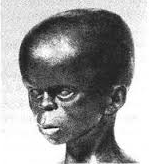
\includegraphics[width=0.50\linewidth]{chast-colebanie-osnov/polane/starosel.png}

\textit{Воссоздание облика «старосельского ребенка». Но дитя ли?}
\end{center} 

В науке идет спор насчет неандертальцев. Одни говорят, что они – предки человека, другие – отдельный вид. И «старосельский ребенок» для первых стал примером «переходного типа» от неандертальца к homo sapiens, для других – помесью, свидетельством естественного скрещивания обоих видов.

«Старосельский ребенок» прочно вошел в книги, статьи. О нем в 1954 году писал даже журнал «Огонек»!

Завершив исследование стоянки, Формозов «законсервировал» ее – как обычно поступают археологи, чтобы никто кроме них не мог изучать памятники старины. Вход в пещеру завалили камнями, те заросли травой, а время от времени сотрудники Бахчисарайского музея смотрели, чтобы туда никто не лазал. Итоги работы Формозов изложил в книжке «Пещерная стоянка Староселье и ее место в палеолите», вышедшей как 71-й том «Материалов и исследований по археологии СССР». 

И вот в начале 1990-х, украинский археолог Виктор Чабай и американский Энтони Маркс провели повторные раскопки в Староселье. Американцы давали на это деньги и получили право брать образцы для изучения. Формозов возмутился. Как, тронули его стоянку? Началась яростная перепалка, в письмах и печати. Подробности опускаю.

«Старосельскому ребенку» нанесли удар. Новые исследователи стали доказывать, что это скелет не древнего ребенка, но похороненный в ближайшие к нам несколько веков татарский ребенок, и странности черепа происходят от дебилизма. Маркс-де нашел поблизости татарские погребения 18 века. Впрочем, Формозов тоже знал о них. И вот ученые принялись ожесточенно спорить, кто прав.

А когда в 2003 году на острове Флорес в Индонезии археолог Майк Морвуд с коллегами нашел останки девяти существ ростом около 1,1 метра и назвал этот биологический вид homo floresiensis, некоторые ученые воспротивились возможности существования подобных существ и возражали – это останки обычных людей, только микроцефалов, да еще кретинов, а если не кретинов, то карликов, или синдром Дауна виноват.

У жителей острова сохранились предания, где этих пещерных волосатых существ называли Ибу Гого. Их встречали вживую еще в 17 веке, когда начали прибывать португальские торговые суда. Местные люди истребили Ибу Гого за похищения человеческих детей и еды. До определенного времени Ибу Гого сосуществовали с людьми. От них маленькие создания иногда получали пищу, могли повторять за ними слова и, скажем так, сочетались браком, ибо длинногрудых жительниц одной из деревень острова считают потомками Ибу Гого.

Когда ученые встречают необычные скелеты, то стараются пояснить находки, исходя из привычных представлений. Так, все небольшие скелеты – дети или подростки. Странный череп? Искусственная деформация!
 
На Урале да в Карелии, народные предания наделяли сгинувший волшебный народ Чудь белоглазую маленьким ростом. В подтверждение тому показывали древние орудия труда небольших размеров. А ведь и на Киевщине находили такие. Археологи в статьях честно отмечают малые размеры и не зря пишут «ножички». Но почему «ножички»? Неужели привычного нам роста люди в здравом уме будут изготавливать себе орудия труда и оружие не по своей руке? Ученые молчат.

В Киеве и окрестностях откапывали скелеты различного роста, с разными очертаниями черепов – в том числе подобные неандертальскому. А. П. Богданов в статье «Древние киевляне по их черепам и могилам» (1879 год) дал обзор черепов – замеры и так далее, и обобщил, что на протяжении веков, высокие, вытянутые назад черепа постепенно сменялись более округлыми. Но разве наука умеет правильно датировать останки? На примере «старосельского мальчика» очевидно, что археологи могут датировать одни и те же останки как сотней тысяч лет до нашей эры, так 18-м веком.

А как насчет Варягов? Если они, как говорят ученые, были скандинавами, то должно быть много «скандинавских» захоронений на той же Киевщине, столице государства, образованного, по мнению норманистов, «викингами». Но здесь вроде ничего  подходящего не сыскалось. Взялись за соседнюю область.

В 19 веке профессор Самоквасов раскопал в Чернигове, за Елецким монастырем, курган Черную могилу (в преданиях связанную с «волшебницей-бусурменкой», провалившейся тут под землю от наперстного креста «владыки» из монастыря) и нашел любопытные вещи, в том числе бронзового литья изваяние 4,5 сантиметров высотой. 

Сидит человечек, держится за длинный свой язык. Теперь археологи говорят – это идол бога Тора, который держится за бороду! Мол, в Исландии и Швеции нашли две подобные костяные фигурки. А раз бородач, значит Тор. Наука заключает – в кургане похоронен Варяг-скандинав. А если бы его погребли с китайским планшетом, получился бы верно китаец. Сам же Самоквасов отметил, что строение кургана совпадает с греческими погребальными холмами «времен Троянской войны». И там лежала византийская монета императора Василия I Македонянина, что относит могилу к временам по крайней мере Вещего Олега. Археологи сделали вывод – здесь был похоронен некий князь, «вождь племени».

Якоже рекохом преже, ученые не понимают давний смысл слова «племя». В свою очередь я, не зная, какой точный смысл вкладывают ученые в «племя», не могу уяснить, что они хотят сказать любимым своим выражением «союз племен». Полян они называют «союзом племен», а Древлян – «племенем».

В летописи говорится о союзе племен? Нет. С чего ученые так решили? Ну наверное, они думают, по-своему разумея, что «племя» – небольшое сообщество людей, живет посёлком в лесу или в поле. А Киевщина большая. Значит, посёлков много, в каждом свое «племя», и нужен их союз.

Как вы себе это представляете? И какова цель создания союза? Договариваются взаимно кланяться при встрече? Делят пастбища и рыбные места? Помогают друг дружке в случае нападения неприятеля?

Ученые не задают себе таких вопросов. Они говорят – союз племен это объединение племен. Единица это один. Лады, что значит объединение? Раньше варили щи отдельно, теперь сообща? Всё имеет устройство. Как должен быть устроен такой союз, какие в нем действуют правила для обеспечения этой «союзности»?

Я, для рассуждений, частично принимаю правила игры ученых. Союз поселений. Не племен, поселений. Надо полагать, что такой союз носит признаки государства. Эти признаки, без которых союзное устройство лишено смысла – общее для подчиненных земель управление, общие вооруженные силы, обложение налогами, и тому подобное. Почему бы науке тогда не признать, что непосредственно до времен Киевской Руси существовали «областные» государства? Ведь и князья их известны – Кий, Хорив и Щек у Полян и Древлян. Потом у Древлян был князь Мал.

В летописях ничего не говорится о «племенах Славян» и союзах таких «племен». Летописи пишут о народах Словенского языка, ветви племени Афета. Название каждого народа согласуется с местом, землями, где живет народ – Поляне, Северы, Древляне. Земли каждого народа и есть «областное» государство, подчиненное крупнейшему городу в крае. 

Сие деление сохранилось поныне. Киевская область со столицей в Киеве – страна и народ Поляне со столицей в Киеве. Черниговская область со «столицей» в Чернигове – Северы со «столицей» в Чернигове. И так далее. Никуда это не делось, только названия и границы отчасти поменялись.

Но ученые нам бают, что жили какие-то племена Славян или даже союзы племен, и вот Варяги, непременно скандинавы, приплывали на своих драккарах и брали дань. 

Художники, внемля сему, рисуют однообразные картины. Берег реки, драккары... А как они, морские да с килями, пристали к берегу? Ладно. Суровые викинги приплыли за данью и вылезли на берег. А там селение, убогие хибары. Запуганные, лохматые Славяне тащат Варягам шкуры, бочки с медом. 

Или, киношники показывают – роща березовая, зелено кругом, птички поют. Сидит Славянин, лапоть плетет. Тут опять же, грозный драккар режет воду выпуклой грудью. Нападение на деревню. Все местные жители – благообразны. С длинными волосами под обруч. Викинги же, косматые, незнакомые с гребнем, из лодей высыпали и ну по сараям шарить. Сальца шматок, мядку туясок! И отбирают последний лапоть, чтобы повезти в Византию и там продать.

Я не утрирую, таково общепринятое представление. Ибо известно, что славянские народы платили дань, а поскольку ученые считают, что общественный строй Славян был на уровне тумба-юмба, то и картина соответствует. Стоящий у истоков российской исторической науки Август Шлёцер в 1809 году писал:

\begin{quotation}
Дикие, грубые рассеянные славяне начали делаться людьми только благодаря посредству германцев, которым назначено было судьбою рассеять в северо-западном и северо-восточном мире семена просвещения. Кто знает, сколь долго пробыли бы русские славяне в блаженной для получеловека бесчувственности, если бы не были возбуждены от этой бесчувственности нападением норманнов.
\end{quotation}

Современные норманисты мало ушли от этого представления, слова только другие! Не так прямо.

Хорошо. Одни платили дань, другие собирали дань. Как происходил сбор дани?

На драккарах много по славянским землям не поплаваешь, хоть это не беспокоит ученых. Перенесем представление о хищническом сборе дани на сушу. Ездили обозом по хуторам, выбивали продукты, шкуры. Это весьма долго, а нагруженный разным добром обоз, колесящий от селения к селению, подвергается опасности куда большей, нежели точечный выезд за собранной в каком-то месте совокупной данью. 

Прочтем кусочек летописи:

\begin{quotation}
В лето 6367. Имаху дань Варязи из заморья на Чюди и на Словенех, на Мери и на всех Кривичех; а Козари имаху дань на Полянех, и на Северех, и на Вятичех, имаху по беле и веверице (по белей веверице) от дыма.
\end{quotation}

Варяги из заморья – подчеркивается, что не просто Варяги, но те Варяги, которые из заморья, а не другие Варяги откуда-то еще – имели дань на Словенах, Мери и Кривичах. А Козари (наука переиначила их в «Хазар») берут дань с Полян, Северов и Вятичей, в размере по «беле и веверице» от дыма\footnote{Значение слова «веверица» было якобы утеряно. Уже в 19 веке предполагали, что это название некоего пушного зверька. В ряде списков про дань сказано: «по беле векше», или «по беле векшице, сиречь кунице». А в одном варианте так: «Варягам с мужа по бели, Казарам с двора по белке». Однако, в украинском языке сохранилось слово вевирка, вевюрка, обозначающее белку. Ваверка, на белорусском, тоже белка. А на румынском veverita.}.

Вдумаемся. Словены (Новгородцы), Мерь, Кривичи платят дань заморским Варягам. Поляне, Северы и Вятичи – Козарам. А как могут платить дань, скажем, все Поляне? Или все Северы? Могут лишь в случае, если они составляют, как бы сказали сейчас, административно-территориальную единицу. Область или, в летописном случае, государство. Ведь сказано в летописи, что дань берется «от дыма». Это значит – с каждого жилья. Подомная дань.

Следовательно, существовал учет «дымов», жилищ. Кто-то вёл этот учет, знал, сколько в каком селении домов. Это было нужно для обложения налогом. В селении таком-то сто дымов. Значит, селение должно выплатить дань в размере 100 умноженное на «белю и веверицу».

Как сейчас собирают налоги – налоговики обозом по квартирам ездят?

Думаю, было как теперь. Каждый двор – дым – выплачивал налог. Относили деньги сборщику налогов. Тот следил за недоимками, и передавал вырученное «выше». А там еще выше. Затем, те же Варяги прибывали в определенное время, в определенное место (коим был защищенный город, столица) и получали свою дань, таким образом уже со всей страны. Как еще можно получить дань с Полян, с Древлян, прочих? Только при наличии держав Полян, Древлян, прочих. Государство знает, сколько в нем дымов и как собрать с них налоги!

Чем же именно платили дань? Шкурками – беля (белка), куня (куница)\footnote{Название «куница» может восходить ко времени Хуннов или Кхунов и тоже быть связано с данью пушниной.}. На миниатюрах Радзивилловской летописи изображена выплата дани именно таким способом – несут пушнину.

Но существует предположение, что все эти куни да бели были названиями монет – например, Вашкевич возводит всё к арабским словам. Однако в старинных документах находим способы оплаты, где ясно указано на оплату именно шкурами, причем арабские слова под все подвести уже не получится. Однако наряду с пушниной упоминаются и монеты.

Выдержка из статута польского короля Казимира III, данного в Вислице, 1347 год – перечисляются различные платы, в том числе «лупежи» горностая, лисицы, барана, куницы:

\begin{quotation}
98. Хто наречет осуженью старостину. Коли кто наганить, а любо нареч.... сказанью старосты Краковского, имеют ему откладать лупежьми горностайными, а старосте Судомирскому или Любельскому ласицами; судьи Краковскому и Судомирскому куницами, подсудком лисицами, подкоморыим по 6 гривен, коморником по 6 шкот, судьями городным по полугривны кождому, земскому писареви кождому по лисицы; а виноватый маеть все платить, нижли будет припущен к другой жалобе.\\

121. О скаранью подсудков. А також уставляем о подсудкох: коли ему нехто наганить, имеет положить любо три вердункы, а любо лупеж лисичий. А тож о судьях о городскых: коли ему хто наганить, имеет положить лупеж бораний, а он то имеет узять, коли свой суд очистит.
\end{quotation}

Стало быть, в самом деле платили шкурами? Известно, что дани были разные, в том числе предметные – например, медом. Но ведь проскальзывает «куница» и в переносном смысле. Были «куничники» – данники. «Кунщик» – сборщик податей. В церковном обиходе, «благословенная куница» – как пишет Даль, «повенечное владыке, пошлина от брака, за второй вдвое, за третий вчетверо». Вкладывался ли переносный смысл в древние подати?

В средневековых завещаниях шкурок нет. Есть монетные деньги. Шкуры, шкурки по завещаниям проходят в составе одежды. Шуба такая-то, некая одежда обшита тем-то. Но предметная дань шкурками, несмотря на множество вопросов, которые возникают у меня, описана источниками.

Предположу еще такое – наложение дани, скажем, «по куне от дыма», подразумевало, что каждый дым должен уплатить деньгами сумму, равную стоимости шкурки куницы. Ведь иначе охотники были бы самыми богатыми людьми, это всё равно что держать свой монетный двор в лесу. Правда, охотничьи угодья имели владельцев, и за незаконные ловы охотники, будучи пойманы с поличным, лишались своей жизни так же легко, как сами лишали жизни зверей.

И неясно мне, по тому же пункту 98 статута Казимира III, почему одним надо платить деньгами, другим – шкурками. Может, название шкурки в то время было уже обозначением определенного количества денег? Скажем, лисица – десять гривен, куница – сто. Это к примеру.

Однако араб Ахмед ибн-Фадлан, путешествуя на Волгу в 921-922 годах в качестве посла к некоему царю Сакалибов (как именовали Славян) Алмушу сыну Шилки, рассказывает о прибытии по торговым делам неких Русов на реку Атыл (отождествляется с Волгой). Эти Русы были высокими, белокурыми. Вот что ходило у них как деньги (русский перевод восстановлен в издании, которое цитирую, по другим источникам, а не переложено из подлинника)\cite{fadlan01}:

\begin{quotation}
Дирхемы Русов – серая белка без шерсти, хвоста, передних и задних лап и головы, [а также] соболи. Если чего-либо недостает, то от этого шкурка становится бракованной [монетой]. Ими они совершают меновые сделки, и оттуда их нельзя вывезти, так что их отдают за товар. Весов там не имеют, а только стандартные бруски металла. Они совершают куплю-продажу посредством мерной чашки.
\end{quotation}

Неясно впрочем, Русы ли это из Киевской Руси? Сведения про весы мне непонятны. Сначала говорится, что весов Русы не имеют, однако у них есть гирьки – «стандартные бруски металла». Как же еще использовать гирьки, как не помещая их на одну из чаш весов? Гирьки, к слову, находят на Киевщине и археологи. 

Далее Ахмед ибн-Фадлан сообщает о мерной чашке, но она пригодна лишь для сыпучих товаров. Не измельчали же все предметы перед совершением сделки, чтобы потом чашкой мерять.  

Значение слов со временем меняется. В древнем своде законов «Правде роськой» (ныне более принято величать ее «Русской правдой») и летописях словом «скот» обозначают, кроме прочего – поначалу скажу осторожно – платежные средства. Вот Повесть временных лет говорит про Ярослава Мудрого, когда тот княжил еще в Новгороде, что для найма войска Варягов, дабы идти выбивать из Киева Святополка и Болеслава, Ярослав делает с новгородцев следующий побор: 

\begin{quotation}
и начаша скот брати от мужа по 4 куны, а от старосте по 10 гривен, а от бояр по 70 гривен; приведоша Варягы, и вьдаша им скот, и совькупи Ярослав воя многи.
\end{quotation}

Здесь скот – и куны, и гривны. А в «Правде роськой» есть например такое:

\begin{quotation}
А от гривне мечнику куна, а в десятину 15 кун, а князю 3 гривны, а от 12 гривну емъцю 70 кун, а в десятину 2 гривне, а князю 10 гривен.
\end{quotation}

Из гривны мечнику идет куна, а в десятину 15 кун, а князю 3 гривны, а из 12 гривен ему 70 кун, и так далее. Здесь из 12 гривен можно отнять 70 кун, и как это сделать, если куны – шкурки, а гривны, грубо говоря – монеты? В том же источнике, за воровство птицы:

\begin{quotation}
А за голубя и за курицу 9 кун, а за утку, гуся, журавля, лебедя 30 резан\footnote{Оставляю толкование слова «резана» в стороне. На древнерусских монетах не найдены надписи вроде «резана», «ногата», «куна», «гривна», столь часто употребляемые в «Правде роськой». На монетах писали просто, нечто вроде – такой-то князь «на столе» (то бишь на престоле, правит), «а се его сребро».}, а штрафа князю 60 резан.
\end{quotation}

Полагаю, девять шкурок куницы стоили бы как-то поболе голубя или курицы, если только штраф не отличается крайней суровостью. 

Я всё же не могу прийти к однозначному выводу о природе «куны», и разнобой источников наводит на мысль, что некогда платили действительно шкурами, но затем слово «куна» употреблялась в переносном смысле, с разной ценностью в различное время. 

Мы говорим «три куска», подразумеваем «три тысячи», а не три куска чего-либо. Сопоставление же ценности одной куны с одной шкуркой куницы, во время действия Правды Роськой, представляется мне сомнительной опять же по размеру штрафа за кражу курицы. Однако более ранняя дань «по куне от дыма» говорит о том, что во время действия этой дани «куна» означала нечто ценное. 

От дани вернемся к данникам. В летописях идет постоянное переподчинение данников. Причем крупных – Полян, Древлян. Такое возможно лишь в случае, когда речь идет о государстве, иначе как сразу переподчинишь раскиданные в каких-то пределах селения?

Итак, Варяги брали дань с Чуди, Мери, Кривичей да Словен, а Козаре – с Полян, Северов и Вятичей. И вот: 

\begin{quotation}
В лето 6370\footnote{По общепринятому способу перевода из лет от сотворения мира на «от нашей эры» – примерно 862 год. Летописи также приурочивают изгнание Варягов ко времени царствования «царя Михаила» – императора Византии Михаила, и при патриаршестве там же Фотия.}. Изгнаша Варяги за море, и не даша им дани, и почаша сами в собе володети; и не бе в них правды, и вста род на род, быша в них усобице, и воевати почаша сами на ся.
\end{quotation}

Варягов изгнали за море, и перестали платить им дань. Это касается только данников Варягов – Чуди, Мери, Кривичей и Словен (Новгородцев). Поляне, Северы и Вятичи остались данниками Козар. Далее:

\begin{quotation}
Реша сами в себе: «поищем собе князя, иже бы володел нами и судил по праву».
\end{quotation}

Решили поискать себе князя, чтобы владел (опять же, получал дань) и судил по праву. «По праву» означает, что князь обеспечивает соблюдение определенного набора законов, «права».

Разные подданные жили по разными «правам». Это хорошо прослеживается в документированной истории, например в 14-15 веках одни живут по Литовскому праву, другие по Немецкому. 

Слово «правда» встарь употреблялось именно в значении «закона». Известен древнерусский сборник законов – «Правда Роська». И любопытно, что в ней четко отделены Роусины от Славян (Словени) – цитирую по древнейшему списку один из пунктов этого свода:

\begin{quotation}
Аж оубыеть моуж моужа то мьстити братоу брата любо отцю сына, любо браточадоу, любо братню сестреви. иже ли не боудеть кто кого мьстя, то положити за голову 80 гривен: аче боудеть княж моужь или тивуна княжа аче ли боудеть роусин, любо гридь, любо коупец любо тивун бояреск, любо мечник, любо изгои, любо словенин, то 40 гривен положити зань.
\end{quotation}

Словом, после убийства, если родичи покойного не хотят мстить смертью, убийца платит им 80 гривен, если жертва – княжий человек или тиун (судья). Однако, если убитый просто «роусин», или купец, или тиун боярский, или мечник, или «словенин», то убийца платит только 40 гривен.

Но вернемся к новгородцам, захотевшим себе князя. Летописец Нестор продолжает Повесть временных лет:

\begin{quotation}
Идоша за море к Варягам к Руси, сице бо ся зваху тьи Варязи Русь, яко се другии зовутся Свое, друзии же Урмане, Англяне, друзии Гте; тако и си.
\end{quotation}

Послали «за море» к народу Руси, что от языка (части племени Афетова) Варяжского. Во время написания строк летописцем, читателю уже не были ясны отношения понятий Варягов и Руси, поэтому летописец поясняет, что именно те (к которым послали) Варяги назывались Русью, так же, как существуют и другие Варяги – Свои (они же Свеи), Урмане, Англяне, Готы.

И летопись ясно указывает на отдельный варяжский народ под названием Русь. Где же обитали Русы?

Норманисты отвечают – вот же, к ним послали «за море». Хорошо. Кто посылает за Варягами? Три народа, что жили от Новгорода до Ростова Великого (под Ярославлем, на озере Неро).

Последнее норманисты не берут во внимание, для них всё крутится возле севера, Новгорода. Оттуда «за море», если понимать буквально, а не как «заграницу» – в самом деле, обращаться можно только на другой берег Балтийского, а там Швеция (Sweden, Svetia, Suetia).

Всегда ли море в летописях это море? Не всегда. Морями называют еще большие озера вроде Ладожского или Чудского. 

%Чудь (не белоглазая) тоже за Варягами посылала. Могла за свое озеро-море послать? Могла.

Согласно некоторым спискам, Днепр «течет из Руси в море теплое, по нему ж живут Варяги» – то бишь Варяги жили и по берегам моря, куда впадает Днепр. Черного. И это уже второе прямое указание на Черное море как на Варяжское – вспомним место, где говорится, что Варяги живут по морю от земель Волошских до предела Симова.

Любопытно уточнение – море теплое.

Этим, во-первых, точным движением лезвия логики отсекается любое море северное, просто по температуре. Во-вторых, летописец знал, какая вода в каком море, для него одно море было теплым, а другое холодным. «По нему ж живут Варяги» – сказано о море теплом. «По нему» – по его берегам, или «по» в значении «за ним», то бишь за ним живут Варяги? В любом случае, в этом отрывке Варяги живут близ Черного моря.

Но допустим, как норманисты говорят, по Варягов посылали за Балтийское море, в Швецию. Вот же Варягов перечисляют: Русь, Свеи, Урмане, Англяне, Готы. Свеями наука считает Шведов. Обосновано ли?

Смотрим карту Bernadus Sylvanus: Quarta Europae Tabula, 1511 год, часть южного побережья Балтики:

\begin{center}
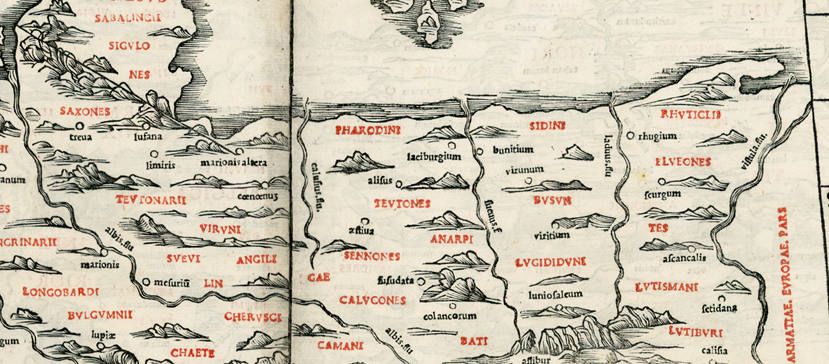
\includegraphics[width=\linewidth]{chast-colebanie-osnov/polane/svevi01.jpg}
\end{center} 

На материке, по реке Albis (Эльба) кучно видим – Svevi, Angili. Кажется, это и есть летописные Варяги Свеи и Англяне. Страна Свэвов – Свэвия. А Свэнами, Свэдами и Свэтами называли скандинавов, обитателей Швеции. Между Свэвами и Свэтами разница величиной с переходной звук четвертой буквы, зависящий от произношения. 

На месте Свэвии ныне – Швабия, южная часть Германии. Кроме прочего, река Шпрее, что течет мимо Берлина, прежде называлась Свэва, а переиначили ее имя крестоносцы. По Свэве жили разные Славяне\footnote{Сохранившиеся в германской области Нижняя Лужица (федеральная земля Брандебург, Niederlausitz, Dolna Łužyca) Славяне – Лужичане (местные Сербы, они же Венды), именуют Шпрею Спрьевьей, а Чехи – Спревой. Спрева – «справа». Как наша Десна, буквально тоже «правая», будет правым, ежели считать против течения, притоком Днепра, так и Спрева будет справа по отношению к Эльбе, куда впадает. 

Чтобы отделять Сербов-Лужичан от Сербов, некоторые именует первых Сорбами, хотя самоназвание их Сербы. Языковед Пол Векслер полагает в Сорбах 9 века предков евреев Ашкенази. В конце 19 века Сорбы-Венды языково сильно онемечились, хотя поныне многие сохраняют славянский свой язык. На 21 век в Саксонии на нем говорят 40 тысяч, в Брандебурге 10 тысяч.

Примеры слов: бахно – болото (ср. с украинским «багно»), байка – сказка, барба – краска (ср. укр. «барва»), беднич – обеднять, бех – бег, бехарка – бегунья, бехар – бегун, блазни – дурень, клоун (ср. укр. «блазень»), божский – божеский, бржух – брюхо, брода – борода, чужба – чужбина, чапка – шапка, дновный – донный, и так далее.}, в том числе Вандалы. Свэвия в европейских хрониках – сплошь и рядом с Галлией, Саксонией, Баварией. 

Кусочек карты 1493 года от Hartmann Schede:

\begin{center}
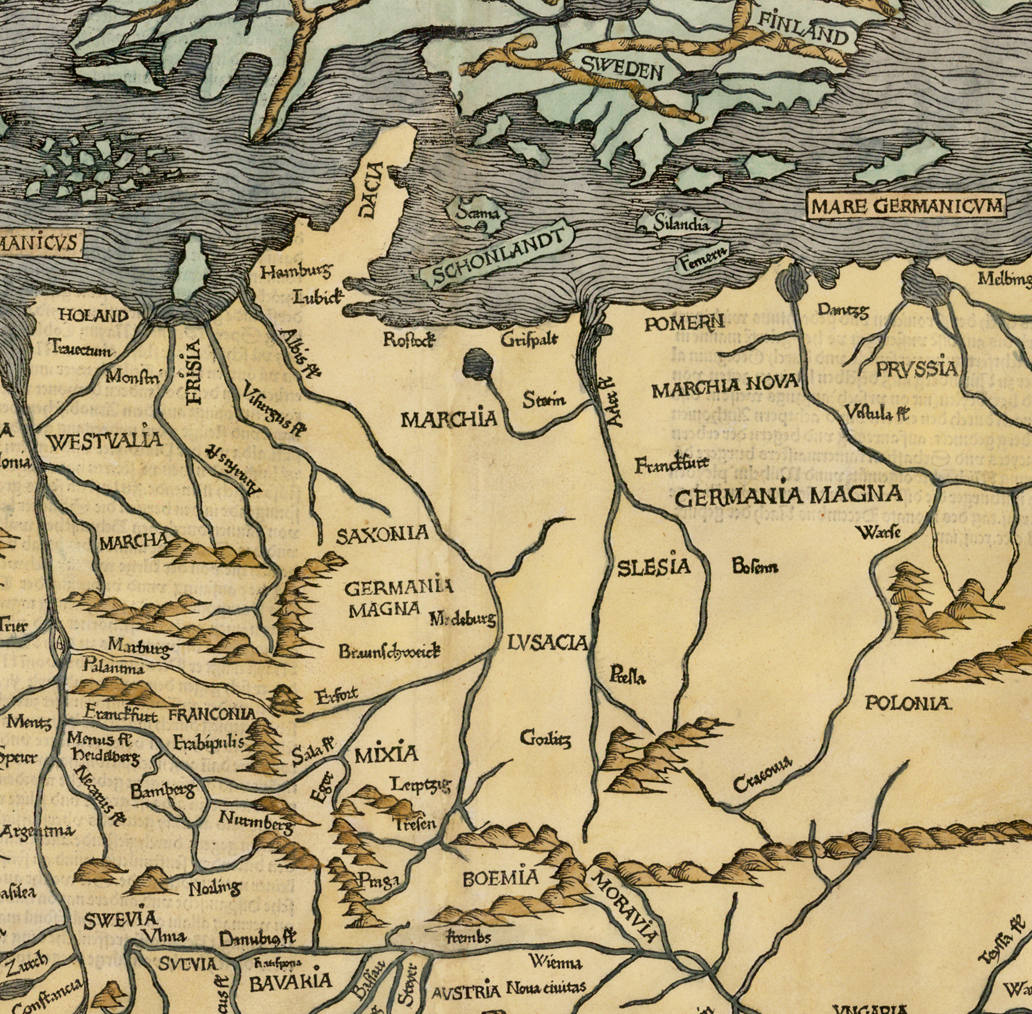
\includegraphics[width=\linewidth]{chast-colebanie-osnov/polane/svevi02.jpg}
\end{center} 

Наверху, на полуострове – Sweden, известная всем Швеция. Внизу слева, на материке, рядом с Bavaria – Swevia, Svevia.

Ибо часть народа Свэвов обитала на материке\footnote{Свэвы жили также в землях нынешней испанской Галиции, примерно откуда, по преданиям Ирландцев, и отправились завоевывать Ирландию люди клана Мила, Скифы-выходцы из Египта. Например, в 6-м веке этой Галицией правил король Мир, а столицей была Брага (теперь относится к Португалии). Мир, брага – понятно без перевода.}, а часть на полуострове, со временем отдаляясь друг от друга в обычаях и речи. Да, полагаю исконных Свэвов – Славянами, что позже онемечились.

В саксонских и смежных хрониках, западноевропейские Аланы, соседствующие со Свэвами, иногда назывались Аламанами (Алеманами), страна же их – Аламанией (Алеманией). Временами она включала в себя Свэвию. Иногда понятия Свэвов и Аламанов смешивались – скажем, «Свэвы» в пределах современной нам Швейцарии были самоназванием, а вот Аламанами их кликали со стороны. 

Теперь земли Аламании лежат в Швабии,  Швейцарии, Австрии и Франции. На страницах хроник, Свэвы, Аланы и Вандалы часто действуют сообща, например захватывают земли Испании. Либо, король Вандалов Крок совместно со Свэвами и Аланами вторгаются в Галлию (части нынешних Франции, Португалии, Испании).% Слово «Галлия» не напоминает вам Алан? А испанская Каталония?

Но что говорят источники со славянской стороны? Чешские хроники много рассказывают о князе Кроке. Польские – о первом короле Лехитов, Краке. У него была дочь, королева Ванда, за которую сватался некий король Алеманов. От ее же имени, согласно преданию из «Большой хроники Полонии» («Chronica Poloniae maioris»), прослыла река Вандал, более известная как Висла, и жители по берегам ее берегов вместо Лехитов прозвались Вандалитами. В «Истории польской» краковского бискупа Кадлубка указана иная причина, что население, бывшее под властью королевы Ванды, стало именоваться Вандалами.

Польский историк, картограф и дипломат 16 века, епископ Вармии, Марцин Кромер в «De origine et rebus gestis Polonorum libri XXX» дает третий вариант возникновения Вандалов. Произведя родоначальника Алана от племени Афетова, далее Кромер с оговоркой «якобы» сообщает, что у Алана было четыре сына, старшим был Вандалом. От него второе имя получила Висла, а Полонов (Поланов, «польских» Полян) назвали Вандалами. Дети Вандала основали королевства Полонское, Русское, Слазское, Моравское, Словацкое, Далмацкое, Паннонийское, Боснянское, Карвакское и Булгарское.

Разве ученые не знают об аланском прошлом Польши, не читали хроник? Знают, читали. Почему же наука продолжает видеть в Аланах «ираноязычные племена», а в Вандалах – «германское племя»?

Но вернемся к Свэвам. Каких Свеев имеет в виду Нестор? На выбор – материковые Свэвы и обитатели Скандинавии, Свэды-Шведы, чей Стокгольм (именуемый на Руси в 18 веке «Стекольня») появился только в 13 веке – много позже Киева, Новгорода, Ростова Великого. А норманисты туда на полуостров, пятью веками раньше посылают за князем, за государственностью.

Кстати норманисты ведут напрасный спор. Как ни крути, население нынешней Швеции – потомки славянских, огульно записанных в германские, народов Свевов, Вандалов, Готов. И если норманисты даже преуспеют в доказательстве своей правоты, вывод по части происхождения Варягов будет одинаковым с антинорманистами! Разница лишь в месте, откуда пришли Варяги Русь.

Но ведь некоторые летописи уточняют их место жительства. Давайте почитаем источники да сравним эти сведения с положением норманистов о том, что призванные княжить Варяги Русь были заморскими скандинавами.

На призыв Чюди, Словен, Кривичей и Веси к Руси княжить откликается Рюрик с братьями:

\begin{quotation} 
Ркоша Русь Чюдь, Словене, Кривичи и Всь: «земля наша велика и обилна, а наряда на ней нет; да поидете княжить и володеть нами». И избрашася трие брата с роды своими, и пояша по собе всю Русь, и придоша к Словеном первее и срубиша город Ладогу, и седе старейшией в Ладозе Рюрик, а другий Синеус в Белеозере, а третий Трувор в Изборьсце. И от тех Варяг прозвася Руская земля.
\end{quotation} 

От возглавляемой братьями Руси (народа из числа Варягов), поселившейся в Ладоге, Белеозере и Изборсце – и земля, где они «сели», прозвалась Руской.

Слово «русский», употребляемое нами теперь для обозначения народа, национальности, прежде носило иное значение. Ведь народы уже имели свои названия. Поляне, Северы, Древляне, Словене, Веся, Мерь, Кривичи. Слово «русский» отвечает на вопрос «чей». Вопрос подчиненности, принадлежности. По мере подчинения этих народов Варягам Руси, народы становились чьими? Рускими, русскими. И земли их тоже именовались русскими. Чья это земля? Варягов Руси, русская.

Прибавляется кое-где в списках, что Вещий Олег был племянником братьев-Варягов, и поселился сперва с Синеусом на «Беле озере», а уж затем Рюрик передал Олегу княжение по смерти своей, покуда сын Рюрика Игорь будет маленьким. 

Согласно летописи, через два года после «призвания Варягов», Синеус и Трувор умерли, не оставив потомства, и Рюрик получил всю полноту власти. Он пришел к озеру Илмерь и построил над рекой Волхов город Новгород (который же вроде уже был построен ранее Словенами), да сделал его своей столицей, а для усиления власти принялся ставить крепости, укреплять селения и насыщать их Русью, хотя исконное население городов было таковым – в Новгороде жили Словене, в Полоцке Кривичи, в Ростове Великом – Меря, на Белеозере – Весь, в Муроме – Мурома. Все эти города стали подвластны Рюрику. Такова обычная, спокойная история по Ипатьевской и Лаврентьевской летописям. Ее признают норманисты.

%\footnote{Ученые относят «финно-угорский» народ Мерь к верховьям Волги. Летописи – к низовьям и Ростову. Там же и окрест жили народы, слывущие как Мэоты, Аланы, Скифы, Роксоланы. Разве науке известно, на каком языке говорила Мерь в летописное время? Как выглядели? Хотя бы имена представителей Мери? Летописи молчат, за них говорят ученые. Есть впрочем на Волге республика Марий Эл, населенная Марийцами, или Чемерисами. По языку ныне они – «финно-угры». Живут Марийцы и на Урале.}, 

А что, если в этих летописях история несколько сокращена? По ряду менее известных списков Повести временных лет оказывается, что Рюрик хотя и «Русь», но «от немец»:

\begin{quotation}
Избрашася от немец три браты с роды своими и пояша с собою дружину многу\footnote{А вовсе не всю Русь.}. И пришед старейший Рюрик и седе в Новегороде, а Синеус, брат Рюриков, на Белеезере, а Траур в Ызборце. И начаша воевати всюду. И от тех Варяг находницы\footnote{Находники – пришлые с чужой стороны и осевшие люди. Некоренное население.} прозвашася Русь, и тех словет Руская земля от рода варяжска, преже быша словяне. 
\end{quotation}

Немцами называли вообще иностранцев из Европы (восточные слыли басурманами). Слово «немец» вроде бы происходит от «немой», говорить по-нашему не умеет. Однако, Немцами именовали и Германцев.

Имена Варяжских Руских князей в разных списках приводятся с отличиями. Трувор: Траур, Труволь, Тривор, Троувыль, Триур, Трубор, Трударь, Триус, Тривус. Синеус (отметим подобие «Триусу» – у одного ус синий, у другого три уса): Синеи, Сенуос. Рюрик: Люрик, Рурик. О Рюрике в «Родословной книге», изданной Беляевым, на пятом листе сказано:

\begin{quotation}
Сей князь Великий Рюрик родом Латынянин из Прусские земли от рода суща Августа кесаря Римскаго\footnote{Augustus, первый император Римской империи. Как считают, жил с 63 года до нашей эры по 14 год нашей эры.}, а колена от Игоря короля обладательства, а от Пруса прародителя своего 14-е колено.
\end{quotation}

Поздняя, 17 века, Густынская летопись, невесть кем сочиненная, соприкоснувшаяся с трудами историков от Птолемея до Стрыйковского и Длугоша, предлагает иной вариант призвания Варягов. Старейшина Словян, то бишь новгородцев, Гостомысл, умирая, повелел подданным идти в Рускую землю, град Малборк, искать там князя:

\begin{quotation}
Нецыи же глаголють, яко Гостомысл, иже бе у Словян, си есть Новгородцов, старейшина, умирая повеле им пойти в Рускую землю, во град Малборк, поискати себе князя; еже и сотвориша.
\end{quotation}

В этой выдержке Руская земля – не привычная нам Русь, а некая исконная земля Русов-Варягов, куда надобно идти из Новгорода за князем. Название Руси потом закрепилось за другой землей, нашей. Что же случилось с прежней землей Руской, где она была?

Malbork, он же ранее Marienburg – город, относящийся к Польше, а ранее к Пруссии. Считается, что основан был в 13 веке. Лежит в 32 километрах на юг от побережья Балтийского моря. Город вроде бы возник вокруг самого большого в мире замка, Малборка (Ordensburg Marienburg). Прусская хроника гласит, что тевтонские рыцари перенесли свою крепость Зантир и дали ей новое имя – Мариенбург, ибо перенесение было совершено в честь Святой Марии.

Но тут 13 век – по общепринятой хронологии. Можно укоротить шкалу датировок. Либо Малборк древнее, чем думают. Я оставляю выяснение истинности дат в стороне.

Слово «Пруссия» похожа на «Русь», да и Рюрик с братьями – «от немцев», а ведь земли Пруссии были захвачены именно Германцами, и летописец мог говорить про Немцев буквально. Малборк и Пруссия упомянуты также в «Сказаниях о князьях Владимирских». Прусский Рюрик выводится там от римского рода цесаря Августа. Да в Степенной книге:

\begin{quotation}
иже начася от Рюрика, его же выше рекохом, иже прииде из Варяг в Великий Нов Град со двомя братома своима и с роды своими, иже бе; от племени Прусова, по его же имени Пруская земля именуется; Прус же брат бысть единоначальствующаго на земли Римскаго Кесара Августа.
\end{quotation}

В знаменитой 16 века «Космографии» Мюнстера вместо южнобалтийской «Пруссии» написано «Русен», точно южнее Мариенбурга (Малборка). 

Когда в фильме «Иван Васильевич меняет профессию» Яковлев произносит: «Рюриковичи мы», это высказывание имеет более глубокую основу, чем кажется. Иван Грозный всем доказывал, что он потомок Пруса, брата Августа. Польша с Литвой смеялись этому, называя «пустыми бреднями», а заодно отрицая существование в прошлом самого Пруса. Ну а наши люди – попробовали бы посмеяться тогда над царем Иваном!

Не стоит однако быть легковерными и принимать за чистую монету всё, что сказано в списках. Ведь если нужно прибавить знатности народу Прусам, то росчерком пера их легко привязать к Прусу, брату Августа. Сей брат неизвестен в дошедших до нас прочих источниках, кроме окололетописных. Где о Прусе и Малборке сказано еще такое\cite[стр. 116]{gilyarov01}:

\begin{quotation}
Сей Кесарь Август разряди\footnote{Распределял владения.} вселенную братии своей и сродников, ему же бяше присный брат, именем Прус, и сему Прусу тогда поручено бысть властодержаство на березех Вислы реки град Мадборок, и Турон, и Хвойница, и пресловый Гданеск, и иныя многия града по реку глаголемую Немон, впадшую в море, иже и доныне зовется Пруская земля. От сего же Пруса семени бяше вышереченный Рюрик и братья его; и егда еще живяху за морем, и тогда Варяги именовахуся...
\end{quotation}

Ко «многия града» есть уточнение: «и Варяжские грады Поморские».

%Сказано, что Август поручил брату Прусу править в указанных городах по берегам таких-то рек, и от Пруса земля та именуется Пруской, а Рюрик и братья – потомки Пруса. Народы, подчиненные Прусу и его потомкам, именовались прускими, прусами.

Имел ли отношение народ Прусы или Пруссы к некоему правителю Прусу – дело темное. Однако такой народ существовал и обитал к югу от Балтийского моря. Под «Прусами» иногда разумеют не название одного народа, но общее обозначение для многих, чьи имена дошли до нас в латиноязычных источниках: Pomesani, Pogesani, Varmienses, Nattangi, Sambite, Nadrowite, Barthi, Scalowi\-te, Sudowite, Ga\-lindite.% (они же ятвиги). 

В современной Литве есть области Pamede, Pagude, Varme, Notanga, Semba, Nadruva, Barta, Skalva, Suduva, Galinda. Любопытно и деление нынешних Литвы и Латвии на «пагастсы», волости. Во времена княгини Ольги и несколькими веками позже, на Руси волости назывались «повостами».

Ученые полагают, что было также отдельное прибалтийское племя Пруссов, по коему стали именовать и остальные племена-народы. В домысле нет надобности. Некоторые германские хроники упоминают Пруссов как отдельный славянский народ, иногда отождествляемый со Сэмбитами.

Иными словами, Пруссами называли то определенный народ, то купно все славянские народы, что жили вдоль южного берега Балтийского моря и на юг, вглубь нынешней Германии. Но помимо «отдельных» Пруссов там обитали и другие славянские народы. В ряде источников «прусские народы» вроде Наттангов отмежеваны от Пруссов. Напротив, говорится, что крестоносцы сначала завоевали те, другие народы, а потом принялись за Пруссов.

Часть былой Пруссии это и современная Беларусь. Там встречаются деревни вроде Пруссы, Малые Прусы, Великие Прусы. Кусок прежней Пруссии – Россия, где Калининград (Кёнигсберг) и от него на юг, запад и восток.

Что же, выстраивается следующие отношения между Варягами, Прусами и Русами. Как понимаю это я следом за летописцем.

На юге Балтики и глубже в материк, обитали одни из Варягов – Прусы либо Русы. Среди них – призванные на княженье деятели Рюрик, Синеус и Тривор. Позже, с распространением влияния Рюриковичей на восток и юг – Ростов Великий, Новгород, Смоленск, Чернигов и вдоль Днепра, в Киев, рускими (а затем «русскими») начали считаться попавшие в подчинение Русам местные земли и живущие там народы. Ветвь Прусов, потянувшаяся за Рюриком, потеряла начальную «п», стала «русами».

А что же исконные «прибалтийские» и «германские» Прусы? Пруссия или Прусия, под этим именем, осталась примерно в летописных пределах, то как герцогство, то королевство (со столицей в Берлине), то часть Веймарской республики. Отваливались от Прусии одни куски, присоединялись другие, а с 1918 по 1945 год «свободное государство Пруссия» было крупнейшей частью Германии, и после победы над Гитлером было поделено между СССР, Германией и Польшей.

Если прусский след в нашей истории верен, то
государственное образование Русь возникло от Пруси. С такими близкими именами они развивались отдельно, а в 1941 году сошлись в смертельной схватке!

На каком языке говорили прусские народы? Многие ученые считают, понимая под Пруссами только прибалтов, что они использовали единый язык, который нынче известен как древнепрусский и относится к западно-балтийской группе. В советское время Владимир Топоров издал пятитомный, составленный по разрозненным немецким источникам и собственному «воссозданию» словарь прусского языка.

Между тем, учитывая неоднородный состав прибалтийских Пруссов (если толковать их как множество народов), возможно, что некоторые прусские народы были Славянами, другие – нет, и используемые в речи наборы слов различались. Вот область Пруссии – Любовия. Это по-каковски? А название прусского замка Рогов – чье слово? А область Самбии – Меденов? Но ученые, как в случае со Скифами и Сарматами, упёрлись – мол, Пруссы это «балты», а не Славяне.

Да что за балты такие? Немецкий языковед 19 века Георг Генрих Фердинанд Нессельман придумал этот термин, чтобы выделить языки Латгалов, Жмудинов, Куршей, Пруссов и других народов Балтики в отдельную группу. И теперь люди думают – балты далеки от славянского рода.

Но берешь даже современные словари например литовского языка, смотришь простые слова обихода. В русском голова, на литовском галва. Русский блин – литовский блинас. Витязь – вытиз. Груздь – груздас. Воля – валя. Двор – дварас. Жернов – жирна. Гром – гриаусмас. Колено – келис. Когда – када. Слава – слове. Снег – Снегас. Степь – степе. Стоять – стовети. Стрела – стреле. Течь – текети. Усадьба – садыба, как в украинском. Успеть – спети. Бегать – бегиоти. Босой – басас. Можно продолжать до бесконечности.

А откроем карту Германии. Южное побережье Балтийского моря, Висмар. Рядом города и селения Бёрцов, Любов, Цуров, Бибов, Гэгелов, Бютцов. Это немецкий? Нет. Прусский язык Топорова? Тоже нет. Это славянские названия.

Ну а вот самая середина Германии, деревня Рута (Rutha)\footnote{50°52'30"N 11°37'14"E}. Мою бабушку Таню немцы туда угнали на сельхозработы во время войны. И мы с ней как-то сели за комп, включили электронную карту и нашли эту Руту.

Захолустный поселок. Мимо протекает речка с названием Рода. По ее течению есть озеро Гибель. От севера к Руте примыкает поселок Лобеда. Неподалеку находятся селения с искаженными славянскими именами Добричен, Цветцен, Буха (Буча), Коспода. Фамилия немецкого баера, хозяина, у которого работали в Руте пленные славяне, была – Висла.

А в окрестностях Берлина есть Тёплиц, Крилов, Далл\-гов-Добериц, Мельхов, Гуссов, Сторков, Шверин, Торнов, Люнов, Готтов, и возле озера Рибенер – поселок Рибен. Нет, на немецком рыба будет не «рибен», а «fisch». Кстати, слово «берлин» славянское, это хорошо известное встарь название лодки\footnote{Даль пишет: «Берлин или берлинка ж. речное судно, по Висле, Днепру и Соже, с острым носом и кормой, до 12 и 20 саж. длины, 2 саж. шир., в осадке 4-6 четвертей, подымающее от 2 до 8 тысяч пудов.»}.

Применительно к прусским землям, окончание немецких селений на «ов», хотя и славянское, однако усеченное, прежде было «ово». Например, было Курово, стало – Куров. Другие преображаются неузнаваемо, как Щекочено стало Закензин, Гако – Шпеком. Окочания же «ин» – это давнее «ино». Ворблино – Варбелин. Наконец, из «ки» у Немцев получилось «ке». Блотки – Блотке. Памятуя эти правила, легко восстановить утраченное звучание\footnote{Подробный этнографический очерк о Славянах южной Балтики Гилдерфинг поместил в пятом Этнографическом сборнике Императорского русского географического общества за 1862 год.}.

Поскольку сейчас там везде живут Немцы, по названиям надо полагать, что прежде там обитали Славяне. И Немцы их оттуда выжили либо подавили, преобразили своей культурой. Как это делалось? Довольно почитать о деяниях Карла, Оттона I и Оттона II, Саксов, а также Тевтонского ордена. Его священник, Петр из Дусбурга в «Хронике земли Прусской» 14 века сообщает\cite{petrdusburg}:

\begin{quotation}
У каждого из этих языческих народов было много крепких замков, которые слишком долго пришлось бы перечислять. Узри же великое знамение Божие и чудеса могущественные! Семь братьев дома Тевтонского с горсточкой оруженосцев, построив укрепление в Кульмской земле на одном дубе, как говорилось, сначала дерзнули выступить против такого огромного и бесчисленного множества язычников, а со временем, за 53 года, перебили их так, что не осталось ни одного, который не подклонил бы выю свою под иго веры, с помощью Господа Иисуса Христа, благословенного во веки веков. Аминь.
\end{quotation}

Судя по описанию обычаев Пруссов в «Хронике» Петра из Дусбурга, это были патриархальные Скифы, не Савроматы. Славянские названия в нынешней Германии, вроде «Рогов» – от Пруссов и прочих славянских народов. Уничтожению язычников-Пруссов тевтонским рыцарям помогали и тогдашние правители соседней Померании, например Святополк II и брат его Самбор, добивавшие Пруссов у реки Сиргун\cite{petrdusburg}: 

\begin{quotation}
Там сверкающий меч воинства христианского насытился плотию язычников, здесь копье не возвратилось, не нанеся ранения, ибо Пруссы ни тут ни там не могли уклониться от лица преследующих, и содеяно было великое избиение народа прусского, ибо в тот день пало более пяти тысяч. После этого все пилигримы с радостью воротились восвояси, восхваляя милость Спасителя.
\end{quotation}

Впрочем, Святополк потом стал «сыном диавола», истребляя уже крестоносцев-тевтонцев при помощи уцелевших Пруссов. Однако вскоре крестоносцы прижали Святополка, и тот вынужден был мириться, отдав «братьям» свой замок, и заложниками родного сына Мстивоя да полководца Вояка.

Адам Бременский, живший в 11 веке, в «Деяниях архиепископов Гамбургской Церкви» широко описывает славянское прошлое нынешней Германии\cite{adambrem}:

\begin{quotation}
Склавания, таким образом, наибольшая область Германии, населена Винулами (Winulis), некогда именуемых Вандалами (Wandali). Десятикратно она больше, чем наша Саксония, если принимать во внимание земли Бомии (Boem\-iam)\footnote{Богемия, часть теперишней Чехии.} и живущих за Оддарой\footnote{Оддара – старое, славянское имя реки, известной ныне как Одр.} Поланов (Polan\-os), ибо одеждой и языком они частично подобны Склаванам. Эта вооруженная, богатая на воинов, плодородная страна с границами, защищенными лесами и реками. В ширину она простирается с юга на север от реки Албии (Albia fluvio)\footnote{Эльба.} до Скифского моря (mare Scythicum). В длину, кажется, начинается в Гамбургском приходе\footnote{Вот имена некоторых славянских князей, приходивших в Гамбург к епископу: Анатрог, Гнев, Ратибор.} и лежит по бесчисленным землям на восток к Бегуарии (Beguariam), Унгрии (Ungri\-am) и Греции (Graeciam).
\end{quotation}

Винулы Адама Бременского, они же Вандалы. Современные ученые говорят про Вандалов, что это – «древнегерманский союз племен». Как видим, сами давние Германцы иного мнения, и относят Вандалов к Славянам. Но что за название – Венулы? Поменяв букву В на Ф и поглядев на карту, где Финляндия, нетрудно догадаться, что Винулы это Финулы.

Почему Финны не говорят теперь на славянском языке? Вероятно, влияние пришлого, иноязычного населения было сильнее, и неясно, сколь много славянства осталось в современных Финнах. Саксон Грамматик в «Деяниях Данов» (Gesta Danorum) пишет кроме прочего о тех еще, исконных Финнах. В книге третьей, Финн со славянским именем Ростов напророчил для Одина, позже обожествленного северянами, что дочь правителя Рутенов, Вринда, родит Одину сына.

Нынешние Финны обозначают Русь (в современном значении, не варяжском) словом «Venäjä» и население ее – «Venäläin\-en». А ведь Винулы-Венулы это прежнее именование самих давних Финнов! Более того, в этом «Веналайнен» слышится искаженное «Аланы». Вспомним и как, по Рубруку, Германцы переиначивали Аланов в Валанов. Сам аланского рода, историк Иордан в «Гетике» отождествляет Аланов и Вандалов – «Vandali vel Alan».

Вильгельм де Рубрук, рассказывая о народе Блак или Илак, живший в земле Ассанов, сообщает про общность языка (речи, набора слов) Илак, Рутенов, Полонов, Боеморов (Богемцев). Язык Склавов тот же, что у Вандалов, пишет де Рубрук на латыни:

\begin{quotation}
Vtrosque enim vocant Ilac, et hos et illos lingua Rutenorum et Polonorum, et Boemorum. Sclauorum est idem idioma cum lingua Vandalorum.
\end{quotation}

Мавро де Орбини приводит небольшой словарик языка Вандалов, составленный по сочинению Карла Вагрийского и «Переселении Народов» Лациуса. Приведу оттуда выдержки, немного переделав словарь под вандало-русский, ибо де Орбини дает переводы на итальянский и местный для него, уроженца Балкан, славянский. 

К сожалению, я не знаком с источниками де Орбини. О Карле Вагрийском ничего не знаю, а про Вольфганга Лациуса (Lacius Hungarian, 1514-1565) известно лишь, что это был венгерский картограф. Соблазнительно мне считать словарь истинным, хотя он – лишь дополнительный довод в пользу славянства Вандалов, в придачу ко свидетельствам давних историков. 

Под «славянством» подразумеваю скорее общий корень, происхождение и речевое сходство. Быть может, Вандалы как народ образовались, когда Славянами никого еще не именовали, или жили себе отдельно Славяне, жили Вандалы, говорили примерно на одном языке, а купно их называли тогда Сарматами или Скифами.

Но вот словарик:

\begin{multicols}{2}
%\setlength{\columnsep}{1.5cm}
%\setlength{\columnseprule}{0.2pt}

\mbox{ }\\
\textbf{Б}\\
\mbox{ }

баба – баба

беда – беда

боти – ботинки

брат – брат

\mbox{ }\\
\textbf{В}\\
\mbox{ }

ведро – ведро

виуно – вино

волк – волк

вуалити – валять

вуйтер – ветер

вунач – внук

вуода – вода

\mbox{ }\\
\textbf{Г}\\
\mbox{ }

голубо – голубь

гроб – гроб

гром – гром

\mbox{ }\\
\textbf{Д}\\
\mbox{ }

дар – дар

десна – десна

дол – дол

дропати – царапать, дряпать (укр.)

дум – дом

дыня – дыня

\mbox{ }\\
\textbf{Ж}\\
\mbox{ }

жена – жена

\mbox{ }\\
\textbf{З}\\
\mbox{ }

звати – звать

зима – зима

зумбы – зубы

\mbox{ }\\
\textbf{К}\\
\mbox{ }

камора – комора

кастан – каштан

кафтан – кафтан

кила – кила

клап – холоп

клатити – колотить

коло – коло

кочка – кошка

круг – круг

кулич – кулич

курвуа – курва

\mbox{ }\\
\textbf{Л}\\
\mbox{ }

леву – лев

лепси – лучший (украинское «ліпший»)

лехши – легкий (украинское: «легший»)

либо – любовь

лисы – лысый

лопата – лопата

лотер – лодырь

луг – луг

люд – люд

\mbox{ }\\
\textbf{М}\\
\mbox{ }

майти – мыть

меч – меч

миликно – молоко

млады – млад

могу – могу

муй – мой

мус – муж

\mbox{ }\\
\textbf{Н}\\
\mbox{ }

наги – нагой

насс – наш

невуеста – невеста

новуй – новый

\mbox{ }\\
\textbf{О}\\
\mbox{ }

олобо – олово

\mbox{ }\\
\textbf{П}\\
\mbox{ }

пасти – пасти, выпасать

перо – перо

пиет – пять

писати – писать

питхи – пить

пламен – пламя

плаути – плавать

плац – плац

плесати – плясать

погити – пойти

покой – покой

потокх – поток

просаш – нищий, проситель

птач – птица, птах

\mbox{ }\\
\textbf{Р}\\
\mbox{ }

работа – работа

розум – разум

\mbox{ }\\
\textbf{С}\\
\mbox{ }

седил – седло

сестра – сестра

сити – сеять

скода – шкода, вред

стати – стать

стол – стол

страч – страх\footnote{Наше «пересрал» – «испугался». Вот где корень!}

схорниа\footnote{От старославянского «скора» – шкура, отсюда «скорняк».} – сапоги

\mbox{ }\\
\textbf{Т}\\
\mbox{ }

танец – танец

теле – теленок, теля

тенета – тенета, паутина

тепли – тепло

тма – тьма

труба – труба

тути – тучи

тэкзаути – танцевать (ср. украинское «танцювати»)

\mbox{ }\\
\textbf{Х}\\
\mbox{ }

хора – гора

хруша – груша

хтити – хотеть (ср. украинское «хотіти»)

\mbox{ }\\
\textbf{Ч, Ш}\\
\mbox{ }

черзи – четыре

шергити\footnote{Вспомним украинские песни-щедривки, когда «засевают».} – сеять
\end{multicols}

Итак, вполне славянский язык, с окончаниями глаголов как в старославянском и украинском, и мягкой «г».

Сигизмунд Герберштейн в своих «Записках о Московии» сообщает, что Немцы называют Вандалами (Vuand\-alis) всех, кто говорит по-славянски. Гельмольд фон Босау в «Славянской хронике» относит Винулов или Венетов, прежде именующихся Вандалами, к Славянам. Ну а польские историки, как мы помним, прямо сопоставляют с Вандалами Полян-леховитов, грядущих Поляков, связав оных с сыном или дочерью Крока, по имени Вандал или Ванда.

Итак, хотя множество источников указывают на славянство Вандалов, а сами Германцы называли Вандалами Славян, нынешние ученые угрюмо повторяют, что Вандалы – «древнегерманский союз племен». Не хочет наука признавать, что Венецию основали Славяне. А ведь от Венеции до страны Словении меньше ста километров!

Не буду затрагивать подробно Готов или Гетов, Мессагетов, Остроготов и прочих, о которых в давние времена много сказано, что говорят они одинаковой речью с Вандалами и Аланами. 

Летопись попа Дуклянина, известная также как «Книга Готская», а в переложении на латынь стала «Славянским королевством». Находим в ней любопытные сведения, что Готы это Славяне, им родственны Вулгары с Волги, а глава Вулгаров зовется «каганом».

К готским народам Прокопий Кесарийский относит Аланов, и утверждает, что готских народов было много, но самыми большими из них слыли Готы, Вандалы и Визиготы, коих прежде называли Савроматами и Меланхленами. Про Вандалов же Прокопий сказывает, что прежде они жили возле Мэотиды, то бишь Азовского моря, вместе с Аланами двинулись ко Франкам, на реку Рейн, затем поселились в Испании.

Полагаю, Вандалы, которые Финны – те же Вандалы, что у Мэотиды и по Висле, только разделенные пространством и временем. Идя через разные земли, они смешивались например с Франками, перенимая их свойства. Известно расселение Вандалов и по Африке, вплоть до Ливии и Мавритании\footnote{Спорю, что их потомки – Туареги, которые в отличие от соседей пользуются ложками, а счет родства ведут по материнской линии – истинно сарматский матриархат. Чадру среди Туарегов носят мужчины, не женщины. Белое население Африки – Берберы да Туареги пользуются письменностью «тифинаг», где многие буквы точно такие же, как в славянском и греческом алфавитах. Немудрено!}. При правителе Вандалов Гизерихе, бок о бок с южными Вандалами сражаются Аланы, вторгаясь в Италию, Сицилию, Грецию, Иллирию.

Традиционные «готские» и «вандальские» имена вроде Аларих, Атилла, Гизерих, Ильдерих звучат вовсе не славянскими. Среди них встречаем и греческое имя Гиларис, и невесть какие Гензон, Год, Аммата, Годигискл, Готфея, Фуския, Гелимер, Оамер и Евагей. Хотя довольно переменить окончание «рих» на «рич» и получим вполне славянское. Было, скажем, Гонорих, а станет Гонорич. Ты чей? Гонорич, от «гонор» производное.

А с Оамером любопытно. Это был племянник правителя Вандалов, Ильдериха (сын Гонориха, а тот – сын Гизериха). Оамер служил своему миролюбивому дяде полководцем и слыл «Ахиллесом Вандалов». После дворцового переворота Ильдерих, Оамер и брат его Евагей были схвачены. Оамера ослепили. Имя его весьма сходно с греческим Омером (Хомером), коего наши переводчики переиначили в Гомера.

Готы появляются на историческом поприще тоже, будто высвеченные вспышкой фонарика. В исторических источниках прослеживаются войны с ними, а потом ррраз – куда-то пропали Готы. То же со Скифами. Раз – и пропали Скифы. Пропасть они не могли, просто их перестали так называть. Теперь это Славяне.
 
Но почему в давних источниках они Склавы или Склавины, откуда этот корень «склав»? Мы знаем, что летописное произношение было через «о» и без «к» – Словене. В основе лежит «слово». А что значит «слово»? Мы знаем слова «слагать», «слагаемое», а значит, «слово» – это краткий вариант «сложенное». Слово из букв сложено, потому и «слово»!

Мы не только «слагаем», но и «складываем». Вот здесь проступает «скл». В русском – «слог», в украинском – «склад» с тем же значением. В каком-то давнем славянском говоре, «слово» звучало как «склово» либо «склаво», потому и Склавы, Склавины. В то время, вероятно в более-менее общем славянском языке, так было. Позже «к» почему-то выпало, склово стало словом, за ним и Склавины превратились в Славян, а вот внешний мир отстал и еще долго писал через «к».

Вернемся к Адаму Бременскому! Он замечает в своем сочинении, что по другую сторону Оддары первыми живут Померани (Pomerani), затем Полани (Polani), от которых далее живут Пруззы (Pruzzos), Бэхэмы (Behemos) и восточные Руззы (oriente Ruzzos). Слово «Померани» восходит буквально к «по морю». Полани – позже Поляки, хотя Полания или Полония это не совсем современная Польша. Менялись границы и население. Например, Полония 15-го века занимала только часть нынешней Польши, лежала южнее тогдашних Пруссии и Литвы. Полани Бременского – такие же Поляне, как на Киевщине, но живущее западнее.

Адам продолжает:

\begin{quotation}
Народы Склавские (Populi Sclavorum) многочисленны, первые соседствуют на западе с  Черезалбийскими Вайграми (Transalbianis Waigri), их город у моря – Алдинбург (Aldin\-burg)\footnote{Алдинбург у Вагров звался Старградом. Не это ли ключ к восстановлению славянских названий?} Затем следуют Ободриты (Obodriti), ны\-не зовомые Ререги (Reregi), и город их Магнополис.

Также перед нами Полабинги (Polabingi) с городом Разиспургом (Razispurg). За ними – Лингоны (Lingones) и Варнабы (Warnabi). Следом живут Хиззины (Chizzini) и Цирципане (Киркипане, Circipani), которые отделены от Толосантибов (Tholosantibus) и Рэтэрей (Retheris) рекой Пан (Panis), город их зовётся Димин (Dim\-ine). Там заканчивается Гамбургский приход.

Другие Скалаванийские народы, обитающие между Альбой (Albia) и Одром – Хэвэлды (Hevel\-di), живущие близ реки Хаболам (Habolam), а также Доксаны (Doxani), Лэубуззы (Leubuzzi), Вилины (Wilini) и Стодэраны (Stoderani). В середине их живут наиболее многочисленные – Рэтарии (Retharii) со своим городом Рэтрэ (Rethre), местом идолопоклонства.
\end{quotation}

Город Димин ныне именуется Деммин (Demmin), а река Пан стала «Пеене». Это сейчас земли Германии. Какие же города окружают Деммин? А вот какие, с очень «немецкими» названиями: Занцков, Рандов, Пензин, Волков, Рустов, Мечов, Гачов, Крукков, Тутов, Фиров, Пасов, Трантов, Медров, Царнеков, Упост, Янков, Доров, Стрелов, Бронков, Раков, Грабов, Грибов, Пустов, Древелов, Буров, Постлов, Куммеров (вероятно от Киммерийцев), Волшов, Гневков, Россин и прочие.

Алденбург теперь зовется Олденбург в Хольштайне (Olden\-burg in Holstein).

Но продолжим читать о Рэтрэ:

\begin{quotation}
Там построен большой храм для демонов, из которых принцем является Редигаст (Redigast). Его золотая статуя – на фиолетовом постаменте\footnote{Кстати, в Византии фиолетовый,  пурпурный цвета считались цветами знати. Прозвище василевса «Порфирогэнэтос» – Багрянородный – означало, что он рожден в особом, обитом пурпуром (порфиром) дворцовом флигеле для императриц-рожениц.}.

У города девять ворот, со всех сторон его омывает глубокое озеро, перейти оное можно по деревянному мосту, через который пропускают лишь тех, кто идет совершить жертвоприношение или спросить ответ\footnote{У гадателей.}. [...] Следующие с этой целью от Гамбурга достигают храма за четыре дня.

За Лэутициями (Лютичи, Leuticios)\footnote{У Титмара Мерзебургского Лютичи кажется то же, что Ободриты и Вагры.}, иначе называемыми Вилзи (Wilzi), течет Оддара, богатейшая река страны Склавании. В ее устье, входящего в Скифское озеро, лежит знатный город Иумнэ (Iumne), благоприятный для стечения с окрестных мест варваров и Греков. О славе этого города сказано многое, однако не всё заслуживает доверия, с удовольствием отмечу несколько вещей. Это действительно крупнейший город на краю Европы, где со Склавами живут другие народы, Греки и варвары. Прибывшие Саксоны (Saxones) получают равное право на жительства, если открыто не объявляют себя христианами.
\end{quotation}

Ретру и Юмну ныне многие ищут, да лишь предполагают. Греки живут в Юмне вместе со Славянами – кажется, вовсе не скандинавы были тогда вездесущи, но Греки да Славяне. Что до Вильцев-Лютичей, то – в выписке из третьей книги второго тома второго русского издания «Славянских древностей» Шафарика, с припиской «у Схолиаста» я обнаружил такое: «Alani lingua earum Wilzi dicuntur crudelissimi ambrones, quos poeta Gelanos vocat» – что значит примерно «На языке Аланов, именуемых Вилзами, говорили жестокие амброны, как поэт назвал Гэланов».

Адам Бременский говорит о жителях Юмны:

\begin{quotation}
Хотя они еще заблуждаются в своих языческих обрядах, нигде более вы не найдете такого честного щедрого и гостеприимного народа. Город богат товарами северных народов, ни одна диковинка там не редкость. Там есть Котел Вулкан (Olla Vulcani), именуемый местными греческим огнем, о нем вспоминал Солин. Нептун проявляется там тройственной природой: три пролива омывают остров, один зеленый, другой белый, течение третьего постоянно бурно.

Из этого города в краткий срок лодки с гребцами добираются, по этой стороне реки, до города Димина (Dyminem), что находится в гавани реки Пэны (Peanis), где также живут Руны (Runi), а далее к области Семланд (Semland)\footnote{«Семланд» переводят в Земландию и отождествляют с местностью, примерно где ныне Калининград.}, которой владеют Прузы (Pruzi). 

Устройство пути таково: от Хаммабурка (Гамбург, Hammaburc) или от реки Албии (Albia)\footnote{Известна ныне как Эльба.} к городу Иумны (Iumne) семь дней пути по суше, по морю же лодками от Слиасвига (Sliaswig) или Алдинбурга (Aldinburc) добираются до Иумны.

На 14-й день пути от города под парусом добираются до Острогард Руззиэ (Ostrogard Ruzzia)\footnote{Острогард Русь – так Датчане именовали  государство, что сейчас называют Киевской Русью. «Остро», возможно, «восток». Адам Бременский отмечает также про Киев: «Haec etiam Chungard appellatur, eo quod ibi sedes Hunnorum primo fuit» – «Также он называется Кунгард, ибо сперва он принадлежал Хуннам».}. В которой столичным городом есть Кивэ (Chive), соперник скипетра Константинополя, светоносного украшения Греции.
\end{quotation}

Кстати, давайте получим представление о германской географии 11 века. Адам Бременский в четвертой книге своего ценнейшего для нас труда подробно описывает Балтийское море и его окрестности. Перескажу, время от времени делая выписки.

Балтийское море или залив, у Адама именуется также Варварским и Скифским. Некие местные жители именуют его Балтийским от слова «балт» или «белт», что переводится как «пояс». Ибо море это, как поясняет сочинитель, словно поясом тянется через земли Скифов до Греции (такое представление сходно с несторовым из описания пути от Варяг в Греки, если там понимать «по тому же морю» как непрерывность Варяжского). У Англичан, Норвежцев, Немцев «belt» значит «пояс», и выходит, именно неславянское население побережья называло сие море Балтийским. А наши летописи именуют его Варяжским. Датчане из своей страны добирались по нему, при попутном ветре, до Острогарда Руси за месяц плавания.

Адам Бременский сначала приводит слова Эйнхарда, что вокруг Балтийского моря живет множество народов, перечисляет их и пускается в дальнейшие пояснения.

\begin{quotation}
Даны (Датчане, Dani) и Свэны (Шведы, Sueo\-nes), которых мы называем Нортманнами (Nort\-man\-nos) – на северном берегу и всех прилегающих островах. Южное побережье принадлежит Склавам (Славянам, Sclavi), Хэйстам (Haisti) и другим разным народам, в особенности Вэлатабам (Welatabi), которых называют еще Вилзами (Wilzi).

Данов и Шведов и прочее население по всей Дании, историки Франков (Francorum) именуют Нортманнами (Nortmann), хотя римские писатели называют так Ипербореев (Yperboreos), много хвалимых Мартианусом Капеллой.

Итак, первыми в устье вышеназванного залива\footnote{То есть Балтийского моря.}, по южному берегу, напротив нас, живут Даны, которых называют Иуддами (Iuddas)\footnote{Страна их популярно известна как Ютландия, б\'ольшая часть Дании. Наука в упор не замечает прямой перевод названия, свидетельствующий, что население исповедовало иудаизм. Среди Датчан много рыжих, Дания расположена относительно близко к Ирландии. Название Дании может быть отголоском Туаха Дэ Дананн. А еще чего? Библейского колена Данова. Хроника 15 века «Chronicon Holsatiae vetus», помещенная в «Accessiones historicae» Готфрида Лейбница\cite{leibn}, отождествляет Данов с библейским коленом Дана, а Иудд, Джутен (Juten) – с иудеями. Что же скажет современная наука? Она совсем забыла написание через «д», для нее Иудды – это Юты, реже Джуты. «Германское племя»! Буковку «т» сделать твёрже – ни-ни! А то ведь будет Юдландия вместо Ютландии, Юды заместо Ютов.}, до озера Слиам (Sliam). Отсюда начинается граница Гамбургского прихода, что через побережье Склаворских народов длится до реки Пан (Panim), где граница нашей епархии (diocesis).

Отсюда вплоть до Оддары обитают Вилзы и Лэутици, а через Оддару обосновались Помераны (Pomera\-nos). 

Далее распространяется большая земля Поланов (Polanorum), которая соединяется с царством Руззиэ (Ruzziae).
%Deinde latissima Polanorum terra diffunditur, cuius terminum dicunt in Ruzziae regnum connecti.

И последней лежит большая область Винулов (Wi\-nulorum provintia)\footnote{Нынешняя Финляндия.}, которая завершает залив. 

Если вернуться к выходу из Балтики с севера, первыми встретятся Нортманны, затем Скониа, область Данов, выше граничит с Готами (Gothi), что живут до Бирки (Bircam). После, на долгое расстояние простираются земли под владением Свэнов (Sueones) до Земли женщин (terram feminarum). Далее следуют Виззы, Мирры, Ламий, Скуты и Турки (Wizzi, Mirri, Lamiy, Scuti et Turci)\footnote{В Финляндии есть город Турку. Современные Финны выводят название этого города от некоего восточнославянского «тургу», торг. Сей старейший город в Финляндии окружен селениями Руско, Руиссало.}, обитающие до Руззии, в которой находится конец залива. Итак, по югу моря расположены Склавы, севером владеют Свэды (Суэды, Шведы, Suedi).

Знатоки тех мест говорят, что возможно добираться из Свэнии (Sueonia) до Греции по суше. Однако сему препятствуют живущие посередине варварские народы, поэтому предпочитают опасное плавание.
\end{quotation}

Далее Адам Бременский подробно перечисляет острова в Балтийском море, говорит, что большинством владеют Даны и Свэны, а некоторыми Славяне. Острова Нортманнов – преимущественно христианские, однако большой Курланд (Churland) выпадает из обоймы, там живут идолопоклонники, у которых много золота и отменные лошади. Курланд переполнен языческими жрецами (divinis), авгурами (auguribus) и нигромантами (nigromanticis)\footnote{Слово «нигромант» составлено из латинского niger – черный, и греческого μαντια (мантия) – прорицатель.}. К прорицателям туда съезжаются со всего света, особенно из Испании и Греции. Впрочем, есть там и христианский храм.

Еще Адам Бременский говорит о другом большом острове, Эстланде (Aestland), около шведской Бирки. На Эстланде не знают бога христиан, а почитают крылатых драконов (dracones adorant cum volucribus) и приносят им в жертву людей, покупая оных у купцов. При этом важно, чтобы у обреченного не было на теле пятен, иначе драконы отвергнут жертву. Сей остров лежит около земли женщин.

Описав «шведские» и прочие острова, Адам переходит к островам напротив славянского, южного побережья. Остров Фэмбрэ (Fembre)\footnote{Ныне он называется Фемарн, Fehmarn.} лежит напротив Вагров (Wagris) и его видно, как и другой остров, Лаланд (Laland)\footnote{Теперешний Loland, огромный остров, лежит к северу от Фемарна.}, из Алдинбурга (Aldinburg). Другой остров лежит против Вилзев (Wilzos), им владеют Рани или Руни (Rani vel Runi), сильный народ Склавов. Адам отмечает, что по закону, их участие обязательно в решении государственных вопросов\footnote{\begin{otherlanguage}{latin}Altera est contra Wilzos posita, quam Rani [vel Runi] possident, gens fortissima Sclavorum, extra quorum sentenciam de publicis rebus nichil agi lex est: ita metuuntur propter familiaritatem deorum vel potius daemonum, quos maiori cultu venerantur quam ceteri.\end{otherlanguage}}. По сему можно догадаться, что тамошние славянские народы имели общее государство, и принимали решения сообща. Возможно, было нечто вроде союза республик. Адам также упоминает о некой дружбе Ранов с богами – и поправляется – «или, скорее, демонами, которым они поклоняются усерднее прочих». Оба славянских острова изобилуют пиратами и разбойниками.

Третий остров, Семланд (Semland), близок к землям Руззов и Поланов (Ruzzis et Polanis), а населяют его Сэмбы или Пруззы (Sembi vel Pruzzi), доброжелательный языческий народ. Адам добавляет, что у Пруззов пострадал за веру бомиорумский (Boemiorum, Богемия) епископ Адальберт (Adalbertus) – не следует путать с архиепископом Адальбертом. Пруззы, по Адаму, мирно уживались с христианскими Германцами, разве что не пускали их ко своим священным рощам да источникам, боясь осквернения. Описаны как синие, краснолицые и волосатые (Homines cerulei, facie rubea, et criniti). Живут в болотах, не терпят над собой господ.

Оставив острова, Адам переносит повествование на материк. Где-то возле южных берегов он помещает Амазонок (Amazonas), обитающих в Земле женщин. Сведения о причине их беременности противоречивы – кто говорит, что это происходит от глотка воды, иные же, что от купцов, или от пленников, живущих среди амазонок, или от каких-то местных чудовищ.

\begin{quotation}
Когда они [Амазонки] рожают, то мальчики выходят Песиголовцами (Cynocephali), а девочки – красивыми женщинами. Они живут вместе, но презирают общество мужчин, а если те приходят, прогоняют их. Песиголовцы – те, кто имеет голову на груди; в Руззии их часто видят пленными, в речи у них слова перемешаны с лаем.

Есть и те, кого называют Аланами или Албанами (Alani vel Albani), себя они именуют Виззы (Wizzi), они – безжалостные амброны (crudelissimi ambrones); от рождения седые; о них пишет Солин (Solinus). Их отчизну защищают собаки. В сражении, собаки выстраиваются в боевом порядке.

Там также есть люди болезненные, зеленые и макробии (macrobii), которых именуют Хусами (Husos), и те, кого называют Людоедами (Antropofagi), ибо едят они человечью плоть. 
\end{quotation}

От других чудовищ, наблюдаемых моряками, Адам Бременский отмахивается, не веря россказням.

Кроме «Деяний епископов Гамбургской церкви» Адама Бременского и «Прусской хроники», любопытствующих читателей отсылаю к «Славянским хроникам» Гельмольда и Арнольда Любекского (это два одноименных сочинения), «Деяниям Саксов» Видукинда Корвейского, а также «Хронике» Титмара Мерзебургского, дабы иметь представления о событиях, приведших к уничтожению и изменению Славян Германии да Балтики.

Относительно мягкое введение христианства на Руси при Ольге и Владимире (как увидим далее в этой книге, Ольга приложила к этому более усилий, нежели Владимир) было, возможно, просчитанным на много лет вперед геополитическим ходом, обезопасившим Русь от посягательств крестоносцев на религиозной основе. Если бы Русь оставалась поганской, у Германцев был бы постоянный повод прийти сюда и предать Славян огню и мечу так, как это некогда делали в пределах нынешней Германии. 

Неужели, однако, убили всех Славян, проживавших прежде в землях современной Германии, Финляндии, Латвии, Литвы, Эстонии? Большая часть уцелела, однако постепенно переменила свою речь, и ныне их потомки от славянства своего открещиваются. Знаменитый арабский ученый ал Хорезми (ал-Хваризми) писал о стране Гирманийи, что это – земля Славян (ас-сакалиба). Сухраб (ибн Сарабийун)\footnote{Наука датирует его сочинение первой половиной 10 века.}, основав свой труд на данных ал-Хваризми, упоминает уже «город ас-Сакалиба Гирманийа» и дает координаты ал-Хваризми 36°40’, 52°00, сопоставлять которые с чем-либо я не берусь. Козьма Пражский в «Чешской хронике» (12 век), обозревая прошлое, вообще сообщает, что Германией именовалась вся земля от Танаиса (Дона) и «до самого запада». В эту-то Германию, «по направлению к северу» Козьма и помещает земли современной ему Чехии.

Славяне ли Варяги Русь? Названия порогов Днепра можно крутить и так, и эдак. Есть еще имена послов от Руси, их мы обсудим позже. Русы в договорах с Византией отмежевываются от Славян, то же различие проводит Константин Багрянородный. По германским источникам, Прусы это, во всяком случае большей частью, народы славянские, да и названия городов говорят про то же. Но Прусы ли Русы?

Вне выяснения последнего вопроса, выстроился более-менее понятный вариант истории. Русы это Прусы, жили в Балтике либо южнее, потом стали княжить где их призвали. На побережье, в современной Германии, существует даже город с названием, схожим с Рюриком – Рерик, в окружении селений с опять же славянскими именами – Панцов, Буков, Речов, Царфцов, Сатов и прочих. Ну что тут поделаешь? И приход Рюрика если не именно отсюда, то из тех краев, кажется мне более обоснованным, чем скандинавское происхождение Варягов Руси.

Если бы не другие, еще более малоизвестные списки, и настойчивая отсылка к Варягам «за море». У  Гилярова находим, например, такое\cite[стр. 114]{gilyarov01}:

\begin{quotation}
В лето 6405-го приидоша словяня из нова града великого торговати за море к Варягам в немецкую область, во град, нарицаемый прусы и рекоше словяне князем варяжским: «земля, господине, наша, рекомая словенска русь, зело добра и обилна всяким угодием, да нет у нас урадников, да не владеет нами никто: поиидите вы, господине, к нам княжити и володети нами».
\end{quotation}

Здесь новгородцы живут в земле, именуемой Словенска Русь, и приглашают к себе из-за моря, от Варягов, из города Прусы, князей. Наш стройный карточный домик еще не разрушается, но покренился. Если верить этому списку, Русь не Прусы.

Много позже в этой книге я сообщу о Прусе и его деятельности вещи, которые внесут полную сумятицу в сказанное ранее.

Не хочу дуть на карточный домик, вытаскивать из него карты, ведь ладно всё получается. Но и у норманистов ладно, если не все летописи читать. Давайте попробуем выстроить рядышком другие домики, из других карт. Для затравки такое.

Мы уже читали, что Рюрик – от Немцев. А был такой молдавский город – Немцы, Немец. В летописном перечислении городов «Руских» (они вынесены отдельно от киевских) сказано: 

\begin{quotation}
На Молдове: Немец на горах, Корочюнов камень, Сочова, Сереть, Баня, Нечюн, Коломша, городок на Черемоши, на Днестре Хотень, то Болгарский и Воложский городок.
\end{quotation}

Посему Рюрик мог происходить из «руского» города Немца. Что за город был и где?

В нынешней Румынии, где есть и «Сочова» (Сучава, Suce\-ava), и прочие города. Около Молдовы, и на части её бывшей территории, до сих пор существует жудец (уезд) Неамц с одноименной рекой, притоком реки Молдовы. Наши современники часто пишут «Нямц», но Румыны произносят «Неамц». Столицей уезда является город Пиатра Неамц, есть там другой город – Таргу Неамц («таргу» – торг, город был торговым), он же просто Неамц.

С летописным утверждением, где Русь выводится от Варягов Русов, мы познакомились. Но есть и другие, тоже летописные утверждения. Например, что Словене, поселившиеся возле озера Илмеря (будущие новгородцы) назвались Руссами по реке Руссе, впадающей в озеро.

Известно такое «Сказание о Словене и Русе и городе Словенске»\footnote{Давнейший список его датируется 1630 годом.}, где, примерно в 3099 год «от Адама» (сотворения мира)\footnote{2409 год до нашей эры, при пересчете по общепринятой формуле.}, либо во время Александра Македонского, действуют скифские князья Словен и Рус. Они с родами своими по какой-то причине покидают отчизну у Эвксинпонта, моря Черного. Бродят, ищут, где бы осесть. И добираются до большого озера Мойска (Словен позже переименовывает его в Илмерь по имени своей сестры).

Волхованье присуждает князьям селиться здесь. Словен основал город Словенск Великий (позже на том же месте или поблизости возник Новгород Великий)\footnote{В одном списке уточняется про устроение Новгорода на другом месте: 

\begin{quotation}
Ныне же Новоград перенесен на ино место от старого града Словена 3 поприща, а на том месте ныне село Митрополье.
\end{quotation}

Поприще – мера длины, бывшая в ходу до версты. Поприще поначалу использовалось при межевании земель и являлось средним расстоянием между поворотами плуга при вспахивании. Оно составляло, по крайней мере на 15 век, 750 саженей. Саженей же разного рода было около десяти, и все разные – от трех до полутора метров. Значит, село Митрополье поглощено современным Новгородом, либо находилось в районе сегодняшних его окраин.}, а Рус обосновался неподалеку от Словенска, построив град Русу, ныне Старую Руссу. Русса, как и Словенск, в свое время пришла в запустение. Её возродили на прежнем месте. На карте это выглядит так – Великий Новгород, к югу от него огромное Ильмень-озеро, и строго на юг от него – Старая Русса, издавна славная добычей соли (при Иване Грозном в ней было 400 соловарень). 60 километров между обоими городами.

По именам князей Словена и Руса стали называться их подданные – Словяне и Русии, Русы.

Предание о Словене и Русе весьма развито в поздних списках летописей. В некоторых остается упоминание про Александра Македонского, однако вместо князей Словена и Руса, «Словены и Русы» выступают то ли в качестве страны, то ли объединения народов. При этом князья их зовутся Великосан, Асан и Авенхасан. Находим в предании даже текст послания к ним Александра Македонского – надо полагать, это перевод, причем судя по языку, века эдак 16-го, с уклоном в земли нынешней Украины:

\begin{quotation}
«Александр, царь царем и над цари бичь божий, презвитяжный рыцарь, всего света обладатель и всех, иж под солнцем, грозный повелитель, к покорным же мне милосердый пощадитель, к непокорным же яростный мечь, страх всего света, честнейший над честнейшими, в далекоразстоятельном и незнаемом крае вашем от нашего величества честь и мир и милость вам и по вас храбросердому народу словенскому, зацнейшему колену русскому великим князем и владцом от моря Варяжского и до моря Хвалимского, велебным и милым мне храбрственному Великосану, мудрому Асану, счастному Авехасану вечне поздравляю, яко самех вас лицем к лицу любезне целую, сердечно приемлю яко други по сердцу моему и нагреднейшии подданицы нашему величеству и сию милость даю вашему владычеству. 

Аще каковый народ вселится в пределех вашего княжества от моря Варяжскаго и даже до моря Хвалимского, да будут вам и потомку вашему подлежимы вечной работе, во иныя ж пределы отнюдь да не вступит нога ваша.

Сие достохвалное дело замкнено сим нашим листом и подписано нашею цысарскою высокодержавною правицею и за природным нашим государьским златокованным гербом привешеным.

Дано вашей честности в вечность в месте нашего дела в Великой Александрии изволением великих богов Марша и Юпитера, и богини Верверы, и Венуса месяца примоса начальнейшаго дня». 

А припинье царские руки верх строк златопернатыми писмены написано сице: 

«Мы Александр, царь царем и над цари бичь, сын великих богов Юпитера и Венуса в небе, земский же Филиппа силнаго царя и Алимпиады царицы, нашею высокодержавною правицею утвердих вечне». 

Сии ж князи словено-рустии, иж таковыя высокия чести сподобишася от всего державнаго того самодержца прияти и сию пречестнейшую епистолию почитаху вельми и обесиша ю в божницы своей по правую страну идола Велеса и честно покланяхуся ей, и праздник честен творяху в началный день примоса месяца
\end{quotation}

Прежде чем двигаться дальше, остановлюсь на любопытной подробности. Я не буду рассуждать, поддельна ли эта грамота. Обращу внимание на другое. Александр ссылается на «греческих», поганских богов, дескать, сказанное в грамоте – с их позволения. Отсылка к богам не редкость и осталась в поговорке «бог в свидетель».

В дохристианское время был обычай, заключив договор, клясться богам. Взамен приносились жертвы. Словно отголосок, что некогда, более сильным существам люди платили за то, дабы те следили за соблюдением договора.

Александр называет себя сыном богов, в частности Юпитера. Юпитер то же, что Зевс. В древности среди Греков нижней дельты Нила и восточного побережья Ливии Зевс совмещался с египетским Аммоном, и в статуях изображался рогатым. Черт с рогами! Языческий бог – в христианстве кто? Черт рогатый!

Так вот, на некоторых древних монетах у Александра Македонского тоже есть рога. Именно эти, «рогатые» монеты отчеканены при Лисимахе, полководце Александра, после кончины императора. Александр называл себя сыном бога, но и сыном земного царя. Следовательно, полубогом. Или, если угодно, полукровкой. Выдающийся полководец и государственный деятель был человеком лишь частично.

\begin{center}
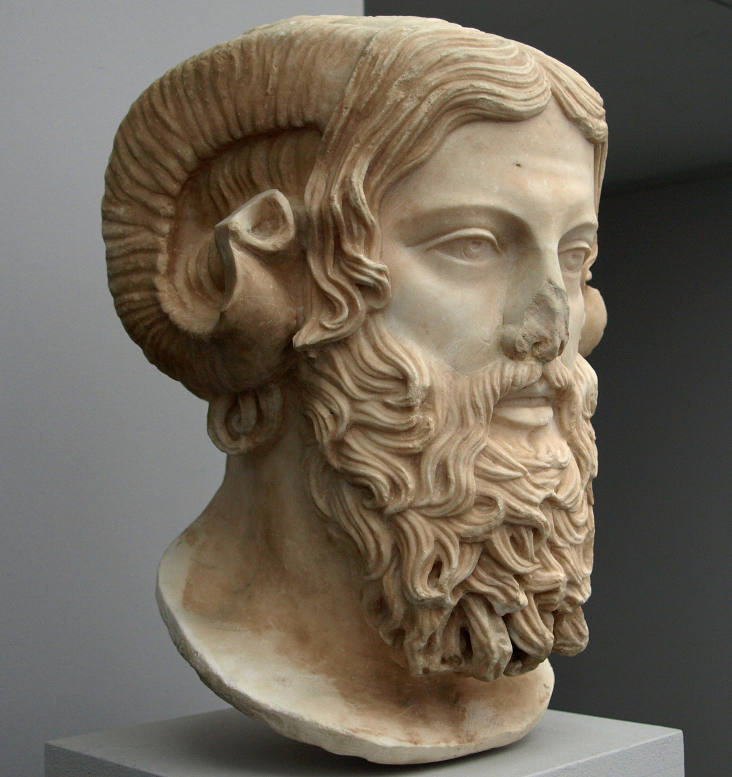
\includegraphics[width=0.40\linewidth]{chast-colebanie-osnov/polane/s-Zeus_Ammon.jpg}

\textit{Зевс Аммон.}
\end{center} 

\begin{center}
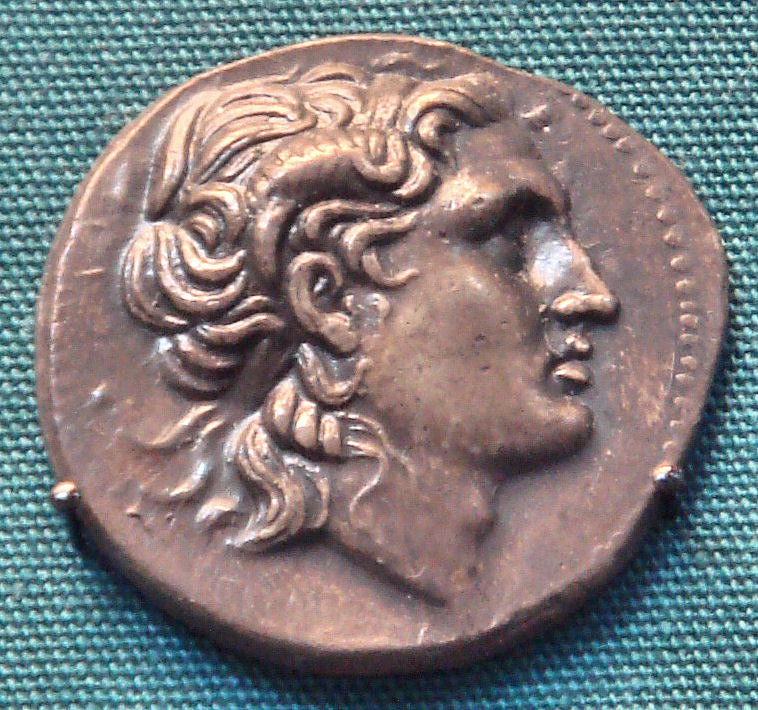
\includegraphics[width=0.45\linewidth]{chast-colebanie-osnov/polane/LysimachusCoinWithHornedAlexander.jpg}

\textit{Монета с Александром Македонским. Фото PHGCOM, сделанное в Британском музее.}
\end{center} 

Александру Македонскому одно время поклонялись, как богу, хотя этот культ получил меньшее распространение, чем почитание Зевса Аммона. Кстати, только ли в Египте да Ливии чтили Зевса? Перун обладает многими свойствами Зевса. Оба – громовержцы. Священное дерево обоих – дуб. Как отмечались празднования в честь Перуна? Неизвестно. Считалось ли, что он рогат? Нет сведений.

Однако на ум приходит образ «вождения козы», приуроченный ко Щедрому или Васильеву вечеру (канун 13 января), к колядованию. Ясно ведь, что это отголосок языческого обряда, от коего осталась, вероятно искаженная, только внешняя сторона. Что же лежало в основе? Не отсылка ли к рогатому божеству? Или жрецы подражали ему своим видом?

\begin{center}
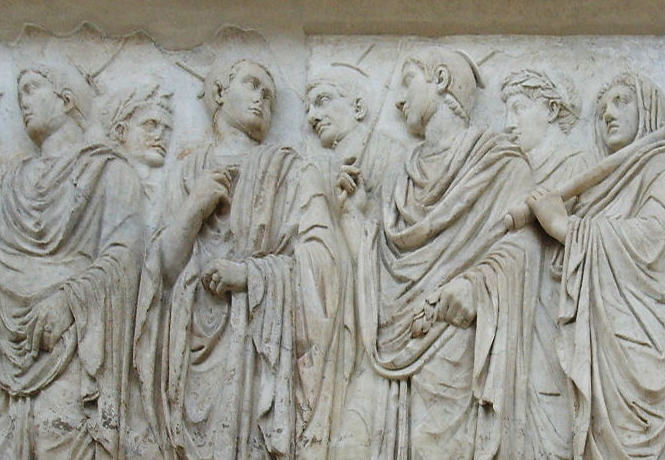
\includegraphics[width=0.70\linewidth]{chast-colebanie-osnov/polane/ara_pacis_fregio_lato_ovest_2_b.jpg}

\textit{Часть рельфа алтаря Ara Pacis Augustae в Риме, датируется 9 веком до нашей эры.}
\end{center} 

В древнем Риме существовала должность Flamen Dialis – главный жрец Зевса-Юпитера. Всего было пятнадцать жрецов, фламэнов, на каждое из верховных божеств. Фламэны носили особые головные уборы («апэксы»), увенчанные «антеннами» (как полагают, деревянными) с пупочкой на конце. Этим жрецам запрещалось выходить к людям либо даже покидать храм без апэкса на голове. Если апэкс хотя бы случайно слетал, жрец переставал быть жрецом. Фламэн Диалис подчинялся большему числу ограничений, чем другие жрецы. Ему нельзя было ходить ночью, касаться лошадей, собак, рыбы и мертвецов, снимать одежду на открытом воздухе, спать вне своей кровати более трех ночей подряд, и так далее. 

Какую еще известную личность изображали с рогами? Библейского пророка Моисея. Известна даже статуя работы Микеланджело в римской базилике святого Петра в веригах (Basilica di San Pietro in Vincoli al Colle Oppio), и многие другие изваяния и картины. В Библии написано, что когда Моисей повторно вернулся с горы Хорив с новыми скрижалями с заповедями взамен разбитых, то не знал, что на голове у него возникли – в подлиннике обозначено «qrn». Аарон и другие израильтяне увидели эти qrn и боялись подойти к Моисею\footnote{Исход, 34:29–30.}.

В русском синодальном переводе вместо «qrn» – лицо Моисея сияет. В церковнославянском переводе – размытое «зрак плоти лица его». Но что за «qrn»? В древнееврейском не писали гласных. Надо догадываться. «Qrn» можно дополнить гласными до  «qeren» – рога. Или до «qeren» – лучи. А также «qaran» – сиял, излучал. Как хотите, так и толкуйте.

\begin{center}
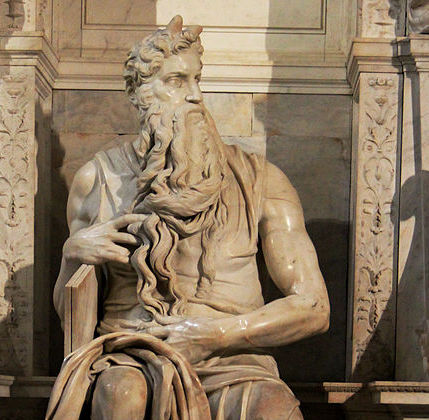
\includegraphics[width=0.60\linewidth]{chast-colebanie-osnov/polane/s-663px-San_Pietro_in_Vincoli_Rome_2011_14.jpg}

\textit{Моисей. Скульптура Микеланджело в Соборе Святого Петра.}
\end{center} 

В Европе, Моисей в скульптурах и на картинах поначалу именно с рогами. А затем, позже – с двумя лучами вместо рогов. Глядя на изваяния Моисеев и не зная заранее, кто это, трудно сказать, Моисей это или Зевс Аммон. А если не видеть нижнюю половину тела, то Пан или сатир.

Но вернемся ко славянским князьям.

Потомки Асана, Авесхасана и Великосана, князья Халох и Лахерн (Алахерн), воевали с Царьградом. Лахерн там погиб (в самом деле, в Стамбуле есть местность Лахерна), а раненному Халоху удалось бежать обратно, да еще с награбленным добром.

Обширный вариант сказания завершается тем, что старейшина Словен (новгородцев) Гостомысл завещает идти за море в землю Прусскую, и призывать на княженье потомков Кесаря Августа. Так, спустя какое-то время по смерти Гостомысла, и призваны были Рюрик с братьями Тривуром и Синеусом, да с ними Олег.

Что до князей Асана, Авенхасана и Великосана, то варианты предания приписывают им создание градов Словенска, Руссы и Суждали\footnote{Есть вариант, где великим княженьем Суждальским владеть, в год 6375 от сотворения мира, начинает Великий Князь Рюрик Африканович, от рода Августа Кесаря Римского.}, а пределы подчиненных им земель простирались не только до Хвалимского, но и Венецийского моря, а также до «восточной страны Сибири». 

И Александр Македонский хотел было идти на них войной, послал угрозу, поминая богов Аполлона, Марша, Юпитера и богинь Вердеру, Венусу и Артемиду. Покоритесь, князья, говорит! Но трое братьев рассудили, что силушки оборониться хватит, и Александру отказали. 

Тот прикинул – воевать далеко, да и условия плохие – леса, болота, водные глубины. Не полез. Выписал пресловутую грамоту на владение землями. Ее повесили в божнице Велеса, причем в городе Ростове Великом. А потом эту грамоту видели в турецком архиве в Стамбуле, прежнем Константинополе. По другим спискам, грамоту получают за военную помощь отцу Александра, Филиппу, а потом и самому Александру.

На след по крайней мере имени такого – Ассан –  можно выйти через описание «Путешествия в восточные страны» Рубру ка, за 13 век. Он пишет, что «Etiam vltra Danubium versus Constantinopolim, Valakia, quae est terra Assani» – за Данубием, против Константинополя, лежит Валакия, которая есть земля Ассанов. Эту землю, по его словам, населяет народ Илак (Блак), у которого язык (набор слов) общий с Полонов и Рутэнов. А поскольку далее Рубрук говорит про то, что язык Склавян и Вандалов одинаков, можно понять, что у Полонов, Рутэнов, Илак он тот же самый. Илак, Блак, Валакия это Валахия. 

Современные ученые, как обычно, отказывают Волохам в славянских корнях, хотя Рубрук, как видим, иного мнения. Он-то слышал их тогдашнюю речь! Да и Нестор отождествляет Волохов с Болгарами, а последние, как известно, пользуются языком славянским.

Повесть о Словене и Русе знает Куманов (Половцев). Они в родстве со Словеном и Русом:

\begin{quotation}
По мале же времени правнуцы Афетовы Скиф и Зардан отлучишася от братий своих и от рода своего от западных стран, и коснушася полуденных стран, и вселишася во Ексинопонте, и живяху тамо многа лета, и от сих породишася сынове и внуцы и умножишася зело, и прозвашася по имени прадеда своего Скифа Скифия Великая. И бысть между ими распря и междоусобица и крамола многа и тесноты ради места. Начальницы же тогда родители их княжаху единого отца сынове пяточислении кровницы, им же имена: первый Словен, вторый Рус, третий Болгар, четвертый Коман, пятый Истер.
\end{quotation}

Таким образом к роду скифову причислены Словене, Русы, Болгары, Команы и Истры.

Разбирая сказание о Словене и Русе, нельзя обойти грамоту, которую, по словам Мавро Орбини, выдал Александр Македонский народу Агриан. Ныне считается, что Агриане «фракийский народ» что обитал севернее Македонии. Есть еще кстати библейские Агаряне – кочевники, производимые от Аврама и Агари, матери Исмаила. Однако на Руси вплоть до 18 века Агарянами кликали тюрков, вообще магометан. 

Но у нас – Агриане. Глава про Агриан называется в переводе книги Орбини так: «О Агрианех народе Славянском Иллирика». Мавро де Орбини пишет – приведу выдержки:

\begin{quotation}
Сии имели жительство между горы Родопа и Ему. Вначале Агриане имели войны неуступные с Александром Великим, и с отцом его Филиппом Царем Македонским. Потом же примиришися со Александром, ясные показали знак своей верности в союзе, хотя развращали некоторые способники Дарию Царю Персскому, неприятелю Александрову: но Агриане и неприсутствующу Александру, под правительством Лагара Царя своего, укротили оную дерзость оных способников, расторгая, и разбивая их полки, обящующе их пребывати в смирении. Александр за сие воздав Лагару достойное благодарение, почтил его драгими подарки, обещева ему в жену сестру свою скоро дати, егда возвратитися в Пеллу. Но оный брак пресече тогда смерть Лагарова с великою печалию Александровую.
\end{quotation}

Тут сведения перекликаются со Сказанием о Словене и Русе двояко. Первое – упомянут «царь Лагар», а в сказании был князь Лахерн. Весомо! Далее, некоторые списки Сказания упоминают о военных заслугах Словен перед Филиппом и Александром Македонским, за что и получили грамоту.

Конница Агриан немало сделала, чтобы помочь Александру разбить войско Дария. Таким образом, Сказание и Мавро говорят об одном и том же, только там Словене, а там – Агриане.

Мавро Орбини продолжает. Он перечисляет, какие страны Александр покорил при помощи непобедимых Агриан, и в благодарность выдал оным грамоту.

\begin{quotation}
Того ради, да признается некаковым образом заслуга Агриан Иллирийских, а во оных и весь род Славянский. Царь Александр дал грамоту жалованную, славную, которую по неско\-льку сот лет некто Иулий Валтасар, секретарь Цесарский, обрел в книгохранилище в Константинополе, в ней же написано сице:

«Мы Александр Филиппович, Царь Македонский, Государь Монархии, изобразительный начатель державства греческого, Великого Диабога сын чрез натавана возвещен обладатель Августов, и брахманов, и арбонов, от Восхода Солнечного, даже до Запада, от Полудни до Севера, благородной породе Славян, и их языку, милость мир, и здравие от нас, и от наших наследников, которые во управлении света по нас наследовати будут. Понеже нам всегда были есте в вере правдивы, во оружии мужественны, и наши проводницы, и силные ратоборцы, за сие вам даем и сообщаем богатодарно, вечно, всю часть земли Северныя, даже до границ последних Полудня Италийского и до гор Персидских, таково, да бы никто дерзал там пребывати, обитати, или жителствовати, разве токмо ваши. А ежели некоторые восходят населятися, да будут вам неволники и дети их, да будут неволники ваших сынов.

Дана во граде Новои Александрии, который основан нами на великой реке Ниле, в лето второе надесять нашего Царствования предстателствующу нам великому богу Иовишу Марсу и Плутону, и богине Минерве. Свидетели сего дела суть высокородный Алцета наш канцлер и прочие единандесят князи, которых по смерти нашей без наследия нашего, оставляем наследниками нашими и всея вселенныя.»

Сия грамота жалованная есть едина от древнейших, какову ни един иный народ вселенныя может показати, во свидетельство мужества наших предков. [...]

Град же Агриа, сущий в Дакии, был создан от сих Агрианов.
\end{quotation}

Что же, очевидно сходство этой грамоты с грамотой из Сказания. Трудно понять, когда было сложено Сказание, вероятно это происходило постепенно, ибо оно соткано из лоскутов. Один из них – либо переделка того же источника, что использовал Орбини, либо напротив, в руки Орбини попала переделка грамоты из Сказания или он он сам переделал текст грамоты. 

Подобная грамота всплывает в «Чешской хронике» Вацлава Хаека (Václav Hájek z Libočan) 1541 года издания, однако доступные мне переиздания выходили значительно переделанными, и редакторы выбрасывали оттуда грамоту, считая ее подделкой. Посему я грамоту из «Чешской хроники» не читал, знаю по отсылкам к ней и сравнить ни с чем не могу.

На фракийско-иллирический след Славена и Руса можно выйти по Татищеву с его палочкой-выручалочкой, «Иоакимовской летописью»\footnote{Татищев говорил, что она древнее Несторовой и написана первым епископом Новгорода, Иоакимом.}, где, в выдержке от самого Татищева, сказано:

\begin{quotation}
Князь Славен, оставив во Фракии и Иллирии около моря по Дунаю сына Бастарна, пошел к полуночи и град великий создал, во свое имя Славенск нарек. А Скиф остался у Понта и Меотиса в пустынях обитать, питаясь от скота и грабительства, и прозвалась страна та Скифия Великая.

После устроения Великого града умер князь Славен, а после него властвовали сыновья его и внуки много сот лет. И был князь Вандал, правил славянами, ходя всюду на север, восток и запад морем и землею, многие земли на побережье моря завоевав и народы себе покорив, возвратился во град Великий.
\end{quotation}

Татищев несомненно обладал такими источниками, что нам и не снились. Между тем «Летопись Иоакима», никем более не виданная, и отрывочно, в пересказе приведенная Татищевым в его «Истории» вызывает у меня ощущение черновика построения исторической модели. 

Грамота Александра Македонского, текстом близкая к той, что привел де Орбини, помещена в Густынскую летопись со ссылкой на чешские хроники. Оная грамота была дана Енетам (Венедам). «Сии же Енеты, или Словяне, иже во Ильлирику», по словам летописца, населили всю Истрию, Далматию, Мисию по обеим сторонам Дуная. Их-то, Енетов, и наделил Искандер грамотой на владение землями аж до северного «океянского Ледовитого моря». 

В Annales Stanislai Orichovi Okszi (17 век), Македонский выдает подобную грамоту князьям (дюкам) Чеху и Леху Роксоланским, причем народы Полоны и Роксоланы в ней различаются.

Нет дыма без огня, и хотя многие исследователи (вообще-то их мало, кого это зацепило) полагают, что «огонь» находится в хронике у Вацлава Хаека и происхождения весьма сомнительного, я не могу строить суждения на столь зыбкой почве.

Чем больше источников мы привлекаем, тем более несуразной и противоречивой получается картина. Суж\-ая набор источников в рассуждениях, мы получаем различные решения «варяжского вопроса». Основных пока – три.

По наиболее узкому набору источников, причем из числа русских летописей, составляется норманская теория. В ней не привлекаются, например, скандинавские саги – потому, что про Рюрика там ничего не сказано. 

Нет и свидетельств, что купцы-скандинавы бойко плавали в Византию, или посещали тамошних василевсов. Основу норманской теории составляет узкий набор летописей, игры с иностранными словами, и находки в курганах предметов, где норманисты усматривают скандинавские черты.

По более широкому набору источников можно сделать вывод, что Варяги Русь – это Прусы, жившие на южном побережье Балтийского моря. Некоторую смуту вносит лишь упоминание «за море». Эта версия с происхождением Рюрика от балтийских Славян кажется мне наиболее обоснованной, если бы я не знал или не хотел замечать остальное. Балтийскими славянами Русью, кстати, могут быть не только Прусы, но и Руги. Помимо юга Балтики и юго-запада Скандинавии, Руги обитали также в Норикуме, откуда Нестор выводит славянский род вообще\footnote{Про Ругов и Норикуме много написано в «Житии святого Северина».}. В давнее время Ругов порой отождествляли с Русами, но верно ли? Однако Прусы – не другое ли, либо измененное имя Ругов?

Огромный – более ста – набор списков Сказания о Словене и Русе позволяет решить «варяжский вопрос» как расширенный вариант с Рюриком от Прусов. Ведь Сказание завершается именно призванием прусского Рюрика, из рода Августа. Уязвимые места здесь – подозрительное сходство Пруса с Русом и производных от них слов, да шаткость составляющих частей самого Сказания. Также сохраняется неопределенность с «за морем». Однако появляется зацепка за скифское прошлое.

Мутный, смешивающее все карты четвертый ответ на «варяжский вопрос» невозможен сейчас, без изложения множества предварительных сведений, посему откладываю разговор до одной из глав части «Киев-Троя». Это новое решение не учтено ни норманистами, ни противниками оных, многому противоречит, многое запутывает, но и проясняет.

Пятый ответ могли бы дать арабские источники 8-12 веков. В них вроде бы хорошо известны континентальные и Русы, и Славяне – я коснусь этого в главе «Град Киев на Лысой», а также некие Русы островные, обитатели островов Азовского (если сопоставление верно) моря. Например, Ад-Димашки в своей космографии пишет\cite{konovalova01}:

\begin{quotation}
Русы называются по имени города Русийа, расположенного на северном берегу одноименного моря\footnote{Море ар-рус, море Русов, оно же Маниташ.}... Они населяют несколько островов в море Манитас и обладают военными судами, на которых ведут войну с хазарами. К ним (русам) приходят по рукаву, текущему в настоящее время от реки Атил\footnote{Волга.}. Когда они идут к главной части реки, то приходят по другому рукаву, текущему в Хазарское море, и нападают [там] на них (хазар).
\end{quotation}

Подобные сочинения несомненно отражают, с той или иной степенью искажения, положение дел в определенное время, но я не буду даже пытаться увязать между собой все источники и наложить их данные на время и место. Моих знаний для этого недостаточно.

Порассуждаю о слове «Варяги». Если проследить упоминания Варягов в летописях и устной речи, то получится следующая картина.

Сначала Варяги предстают народами, живущими по берегам Варяжского моря. Летопись умалчивает, какие именно Варяги облагали данью Словен, Чудь, Мерь и так далее. Однако данники смогли изгнать Варягов «за море».

Затем Варягов, а именно знатных представителей народа Русь, приглашают княжить. Словены и другие уже не просто становятся данниками, но «встраивают» в себя загадочный варяжский народ Русь, превращаются в «русских».
 
Далее в летописях Варяги, без указания их народности, изображены как наемники, обычно приближенные к князьям.

Владимир Красно-Солнышко приходит к Новгороду «с варягами». Много позже «в лето 6523 хотящу ити Владимеру на Ярослава, сына своего. Ярослав же посла за море и приведе варяги, бояся отца своего» – уже сын Владимира Ярослав нанимает за морем Варягов, опасаясь своего отца. Сказано в летописи еще такое: «Уведавши же Святополк, яко еще дышит (князь Борис), посла два варяга прикончить его». Не просто «два вои», а именно два варяга. Нанятые варяги служили князю.

Становится понятной украинская поговорка «скачи, враже, як пан скаже». С чего бы врагу плясать для пана?

Не потому ли, что слова «враг» и украинское «ворог» – то же, что «варяг»? Пословица сохранила представление о назначении, функции варягов. Только в таком значении – наемный человек – она имеет смысл.

Слово «враг» появляется в летописях в годы, когда слово «варяг» уже не употребляется. Никто этой странности не замечает. Когда в летописи исчезают упоминания о варягах, язык летописный обогащается словом «враг», причем в значении «неприятель». Это значит, что, во-первых, к тому времени варяги-наемники, успев насолить народу, воспринимались отрицательно. Во-вторых, варяги именно как наемники отошли в прошлое.

А кем они стали? Откроем словарь Даля: 

\begin{quotation}
Варяг м. скупщик всячины по деревням; маяк, тархан, орел; или кулак, маклак, прасол, перекупщик; или офеня, коробейник, щепетильник, меняющий мелочной товар на шкуры, шерсть, щетину, масло, посконь и пр.
\end{quotation}

Подобно тому, как некогда воинственные запорожские казаки оседали, занимались торговлей, так и варяги наверное превратились в перекупщиков. 

Какие еще слова русского языка напоминают о варягах? Варежка – вязаная рукавица. В словаре Даля есть вариант – варьга. Кроме прочего, варежки в старину надевали под кожаные рукавицы. Но при чем тут Варяги, я не знаю. Может, им были присущи вязаные рукавицы, и потом такие в народе стали звать варежками.

Вновь обратимся к Далю – он пишет про архангельское словцо «варяжа»:

\begin{quotation}
ВАРЯЖА об. арх. (Варяг?) заморец; заморье, заморская сторона.
\end{quotation}

Вместе с тем, по Далю, «Варяга» – это «вор». Но что же, всё население вокруг моря воровало? 

Отметим – самих Варягов никто не грабит. Они облагают других данью, участвуют в военных действиях как наемники. Но кроме известного случая «изгнания за море» Варягов, их больше не трогают. Вроде должны быть богатыми. Но когда какому-то князю хочется воевать, он идет на Новгород, на Киев, «на Козаре», «на Греки» – куда угодно, только не «на Варязе». Причем, чаще всего в составе «воев» княжеских непременно есть эти самые Варяги.

Думаю, слово «варяги» в каких-то участках летописи вообще означает уже наемника в чистом виде, без привязки к географическому происхождению. Возможно также, что в определенных местностях варяги стали уже местной военной кастой, подобно детям боярским, казакам, стрельцам.

Раньше я предполагал, что варяг – от слова «варта», стража. Что значит слово «варта»? Караул меняется по кругу, «вертается», вращается\footnote{Можно продолжить сопоставления. Варяг-торговец всё время крутится, у него оборот, вращение товаров и денег. А слово «варить» – когда мы варим, мы помешиваем, вращаем. У «варить» и «вращать», наверное, общий по смыслу корень.}. Варяг – тот, кто стоит в варте, в карауле, стражник, телохранитель. Варягами примерно в этом значении  окружали себя не только наши князья, но и византийские императоры.

Сейчас я придерживаюсь следующего толкования «варягов».

Поможет разобраться буква «г». Латинский её вариант «g» сохранил чудесное свойство читаться то как «г», то как «дж», «ж». Наше «г» в окончаниях тоже переходит из «г» в «ж». Острог – но сторожить, сторожа. Бог – боже, друг – друже, враг – враже.

Вот это ближе. Враже. 

В летописях никогда не говорится «варяги». Согласно языку летописей, это «варязи». 

А всем знакомо слово «ружьё». Что оно значит? Далеко ходить не надо. Ружье что делает? Разит, поражает.

В украинском языке есть слово «вражати» – поражать. Что же делают «варязи»? Вот и разгадка.

Норманисты, доказывая свою правоту, часто ссылаются, особо не вникая в подробности, на скандинавские саги\footnote{Вариант этой главы с подробным разбором таких саг был мною утерян, снова поднимать источники у меня нет сил, поэтому делаю по памяти краткую выжимку.}. 

В самом деле, там есть некие варингьяры (vaeringjar), весьма созвучные с Варягами. Но варингьяры эти встречаются в сагах только как царская стража в Константинополе! Из прочитанных мною саг, только в одной рассказывалось именно про скандинава, который, прибыв в Константинополь, поступил на службу в эту стражу и дослужился там до высокого чина.

%\begin{center}
%\includegraphics[width=\linewidth]{chast-colebanie-osnov/polane/Skylitzis_Chronicle_VARANGIAN_GUARD.jpg}

%\textit{Стража Варангов, иллюстрация 12 века из мадридской версии рукописи Joannis Scylitzae Synopsis Historiarum.}
%\end{center} 

Странное дело – варингьяров в Скандинавии нет! Наши летописцы помещают Варягов по морю Варяжскому, а саги да византийские источники помещают варингьяров и βάραγγοι (вараггои) в Константинополь, на стыке Черного и Средиземного морей. Это еще одна монетка в копилку догадок, что летописное Варяжское море может быть и Балтийским, и Средиземным. 

К сожалению, в научных работах, разных энциклопедиях и прозе к Варягам относят летописных персонажей, не имея на то оснований. Например, Вещий Олег вторично посылает к Грекам послов, установить мир. В летописи перечислены имена послов, но не сказано, что это Варяги. 

Имена таковы, по Ипатьевскому списку: Карлы, Инегелд, Фарло, Веремоу, Рулав, Гоуды Роуад, Карн, Фрелав, Руал, Актеву, Труан, Лидоу Фост, Стеми. И вот их уже считают Варягами, исключая впрочем тех, у кого проскальзывает некий славянизм.

Но летопись не называет этих послов Варягами. Летопись не говорит, что Варяги – скандинавы.  Более того – у меня греческое имя, но я не Грек. А возьмем дворянство России в 19 веке, которое французский знало лучше русского, да имена себе брали под стать – всякие там Пьеры да Жюли. Они французами, что ли, были? 

А если договор попал в летопись из копии на греческом языке, с искаженной передачей имен?

Но в разного рода литературе вопросы вообще сняты – там вышеупомянутые послы давно стали действующими лицами произведений, персонажами-Варягами, причем особенно полюбился сочинителям Веремуд. Еще с 19 века. Был такой писатель, Александр Красницкий, Веремуд у него действует в романе «Князь Святослав» – уже тогда писали прозу, где все кричат в рупоры нарочито старинными словесами.

Есть еще более внушительный список послов в договоре уже Игоря с Греками. И этих послов, у кого из норманистов доходят руки, тоже записывают в скандинавы.

Между тем и антинорманисты судят поверхностно, трактуя летописное:

\begin{quotation}
А Словенеск язык и Рускый один; от Варяг бо прозвашася Русью, а первее беша Словене; аще и Поляне звахуся, но Словенская речь бе. Полянми же прозвашася, занеже в поле седяху; язык Словенескый бе им един.
\end{quotation}

Антинорманисты здесь усматривают отождествление языков – наборов слов. В то время как Нестор указывал на тождество названий одного народа. Мол, сперва беша Словене, Полянами еще назывались, и была у них речь Словенская. А потом, от Варягов Руси, Словенский язык (язык племени Афета) прозвался Русью.

Вообще происхождение народа Руси, подмявшего под себя Славянские народы и как бы растворившегося в нем – загадка. 

Ломоносов справедливо рассуждал, что в нашей речи должны были остаться слова этих Русов. Однако «скандинавских» слов нет, хотя полно тех, которых, как считается, мы набрались от скажем Татар, соприкасаясь с ними исторически. 

Возможно, Русы были весьма совместимы со Славянами по набору слов, будучи некой ветвью Скифов и (или) Сарматов. Вместе с тем, судя по отрывку о порогах у Константина Багрянородного, Славянские названия порогов мы можем понять куда лучше, нежели Росские.

В Повести временных лет есть любопытная тонкость – когда Вещий Олег заключил первый договор с Греками, то кроме прочего обязал тех: 

\begin{quotation}
«исшийте парусы паволочиты Руси, а Словеном кропиньныя», и быть тако; и повеси щит свой в вратех, показуа победу, и поиде от Царяграда. И воспяша парусы паволочиты, а Словене кропиньны, и раздра я ветр; и реша Словене: «имемся своим толстина, не даны суть Словеном пре».
\end{quotation}

Здесь, в походе Олега, народы Русь и Словене, войска их на кораблях, выступают союзно, однако раздельно. И для Руси приказано шить парусы «паволочиты» (шелковые), а Словенам «кропиньныя» (не знаю уж, что значит, но предполагаю, что подешевле). И ветер разорвал, «раздра» эти кропиньныя парусы. Тогда Словене сказали, мол, поднимем \textbf{свои} толстины – грубые, холщовые парусы, раз не даны Словенам новые паруса. В договоре же с Византией речь идет об отношениях Русов и Греков, про Словен молчок, они вне договора.

Но многие имена послов Олега, вроде Карлов да Инегелда в самом деле какие-то неславянские, от них таки веет севером. 

А имя Рюрик похоже на Рорик, тоже бывшее в ходу у северян, в частности известен король Данов или Юдов Рорик, дед Амлета – ведь Шекспировский «Гамлет» имеет историческую основу. Хотя если выстраивать происхождения, исходя из имен, то выйдет, что Петр I был Греком.

Что до «скандинавского» звучания имен Рорик и Рюрик, то давайте сравним. Саксон Грамматик в книге пятой приводит имя правителя Склавов (Славян) – Струник (Strunico, Sclavorum rege). То же окончание, что в «Рюрик». При этом Грамматик отличает Склавов от Рутенов (Ruthenos) – последние живут в Русции (Ruscia). Имена двух правителей Рутенов – Олимар и Даг. Олимар величался также «правитель Восточный Олимар» и «король Олимар» (rex Olimar). Побежденный Олимар был послан Данами в Свэтию (Suetiam), а позже назначен ими же префектом Холмгарда.

В Персии властвовал Исдигерд – тоже скандинав?

Откроем Патерик Печерский, «Сказание о святей чудотворней церкви Печерской каменной оуспения пресвятыя Богородицы». Начинается оно так:

\begin{quotation}
Бысть в земли Варяжской князь Африкан, брат Якуна слепого\footnote{Якун упоминается в Повести временных лет.}, сему Африкану бяху два сына Фрианд и Шимон: по смерти же отца их изгна Якун обоих о области их. Прииде оубо в Россию Шимон ко благоверному князю Ярославу [...]\end{quotation}
 
Спустя некоторое время Шимон пришел в Печерский монастырь, где стал Симоном и подарил Феодосию Печерскому «имения многы» на строительство церкви.

\begin{quotation}
И понеже бысть прежде Варягом, [...] остави Латинское буйство, и истинно восприя православную Христову веру со всем домом своим, в немже бе яко до трех тысячь душ, и со иереи своими.
\end{quotation}

Так что, варяжские имена Африкан и Шимон –  скандинавские? У католика Шимона имя иудейское, означает в переводе «услышанный». Симеон – греческий вариант Шимона. Африкан – в переводе с латыни значит «африканец», значит это было прозвище. Хорош скандинав!

Призыв на княженье Рюрика иногда кажется мне странным, иногда нет. Во времена сомнений я допускаю, что Рюрик с братьями просто воспользовался междоусобицами Словенов, Чуди, Мери, чтобы захватить власть – и для облагораживания сего, в Повесть временных лет позже был добавлен кусочек о «призвании». В одном списке, в полном согласии с понятиями нынешних норманистов, сказано, что Варягов умоляли прийти княжить: «они же бояхуся зверинаго их (славян) обычаа и нрава, и едва избрашася три браты».
 
Предание о «призвании» Рюрика словесно узаконивает его и его потомков власть. И ничего-то у нас нет больше из источников, кроме этого летописного.

По летописям приходится судить и о первых князьях в Киеве. Первых в том смысле, что сведения о предшествующих не сохранились. Здесь тоже, как в случае с «призванием Варягов», путаница начинается сразу же, стоит сделать шаг в сторону от общепринятых представлений.
